\documentclass{beamer}\usepackage[]{graphicx}\usepackage[]{color}
%% maxwidth is the original width if it is less than linewidth
%% otherwise use linewidth (to make sure the graphics do not exceed the margin)
\makeatletter
\def\maxwidth{ %
  \ifdim\Gin@nat@width>\linewidth
    \linewidth
  \else
    \Gin@nat@width
  \fi
}
\makeatother

\definecolor{fgcolor}{rgb}{0.345, 0.345, 0.345}
\newcommand{\hlnum}[1]{\textcolor[rgb]{0.686,0.059,0.569}{#1}}%
\newcommand{\hlstr}[1]{\textcolor[rgb]{0.192,0.494,0.8}{#1}}%
\newcommand{\hlcom}[1]{\textcolor[rgb]{0.678,0.584,0.686}{\textit{#1}}}%
\newcommand{\hlopt}[1]{\textcolor[rgb]{0,0,0}{#1}}%
\newcommand{\hlstd}[1]{\textcolor[rgb]{0.345,0.345,0.345}{#1}}%
\newcommand{\hlkwa}[1]{\textcolor[rgb]{0.161,0.373,0.58}{\textbf{#1}}}%
\newcommand{\hlkwb}[1]{\textcolor[rgb]{0.69,0.353,0.396}{#1}}%
\newcommand{\hlkwc}[1]{\textcolor[rgb]{0.333,0.667,0.333}{#1}}%
\newcommand{\hlkwd}[1]{\textcolor[rgb]{0.737,0.353,0.396}{\textbf{#1}}}%
\let\hlipl\hlkwb

\usepackage{framed}
\makeatletter
\newenvironment{kframe}{%
 \def\at@end@of@kframe{}%
 \ifinner\ifhmode%
  \def\at@end@of@kframe{\end{minipage}}%
  \begin{minipage}{\columnwidth}%
 \fi\fi%
 \def\FrameCommand##1{\hskip\@totalleftmargin \hskip-\fboxsep
 \colorbox{shadecolor}{##1}\hskip-\fboxsep
     % There is no \\@totalrightmargin, so:
     \hskip-\linewidth \hskip-\@totalleftmargin \hskip\columnwidth}%
 \MakeFramed {\advance\hsize-\width
   \@totalleftmargin\z@ \linewidth\hsize
   \@setminipage}}%
 {\par\unskip\endMakeFramed%
 \at@end@of@kframe}
\makeatother

\definecolor{shadecolor}{rgb}{.97, .97, .97}
\definecolor{messagecolor}{rgb}{0, 0, 0}
\definecolor{warningcolor}{rgb}{1, 0, 1}
\definecolor{errorcolor}{rgb}{1, 0, 0}
\newenvironment{knitrout}{}{} % an empty environment to be redefined in TeX

\usepackage{alltt}

\def\currentCourse{An introduction to graph analysis and modeling}
\def\currentInstitute{Julien Chiquet}
\def\currentLogo{../common_figs/logo_imperial}
\def\currentDate{February, 2019}
\def\currentChapter{Descriptive Analysis of Network Data}


% THEME BEAMER
\usepackage{../beamer_theme}

\graphicspath{{figures/},{../common_figs/}}

\usepackage{multirow}
\usepackage{tikz}
\usepackage[vlined]{algorithm2e}

\pgfdeclareimage[width=.5cm]{computer}{computer.png}

\title{\currentCourse}

\subtitle{\huge\currentChapter\normalsize}

\institute{\currentInstitute}

\date{\currentDate}



\AtBeginSection{
  \begin{frame}<beamer>
    \frametitle{Outline}
    \framesubtitle{\insertpart}
    \tableofcontents[currentsection,currentsubsection, subsectionstyle=show/shaded/hide]  
  \end{frame}
}

\AtBeginSubsection{
  \begin{frame}<beamer>
    \frametitle{Outline}
    \framesubtitle{\insertpart}
    \tableofcontents[currentsection,currentsubsection, subsectionstyle=show/shaded/hide]  
  \end{frame}
}

\AtBeginSubsubsection{
  \begin{frame}<beamer>
    \frametitle{Outline}
    \framesubtitle{\insertpart}
    \tableofcontents[currentsection,currentsubsection, subsectionstyle=show/shaded/hide]  
  \end{frame}
}

\newcommand{\dotitlepage}{%
  \begin{frame}
    \titlepage
    \vfill
    \begin{center}
        \scriptsize\url{https://github.com/jchiquet/CourseNetworkLondon}
    \end{center}
    \vfill
    \includegraphics[width=2cm]{\currentLogo}\hfill
    
\includegraphics[width=2.5cm]{logo_inra}
  \end{frame}
  %
}

\newcommand{\dotoc}{%
  \begin{frame}
    \frametitle{Outline}
    \tableofcontents[currentsection,
    sectionstyle=show/show,
    subsectionstyle=hide]
  \end{frame}
  %
}



\usetikzlibrary{calc,shapes,backgrounds,arrows,automata,shadows,positioning}
\IfFileExists{upquote.sty}{\usepackage{upquote}}{}
\begin{document}

\dotitlepage

\begin{frame}
  \frametitle{Outline}
  \tableofcontents[hideallsubsections]
\end{frame}

% \begin{frame} 
%   \frametitle{References}
% 
%     \begin{thebibliography}{99}
%       \setbeamertemplate{bibliography item}[book]
% 
%     \bibitem[EK2]{EK2} Statistical Analysis of Network Data: Methods and Models, 
%     \newblock \textcolor{black}{Eric Kolazcyk}
%     \newblock \alert{Chapiter 4, Sections 2 and 3}
% 
%     \bibitem[EK1]{EK1} Statistical Analysis of Network Data with \texttt{R}, 
%     \newblock \textcolor{black}{Eric Kolazcyk, G\'abor Cs\'ardi}
%     \newblock \alert{Chapiter 4, Sections 2 and 3}
% 
%       \setbeamertemplate{bibliography item}[article]
% 
%     \bibitem[CM1]{CM1} Analyse statistique de graphes, 
%     \newblock \textcolor{black}{Catherine Matias}
%     \newblock \alert{Chapitre 2}
% 
%     \end{thebibliography}
% 
% \end{frame}

%% ==========================================================================
\section{Basic notions on graphs and networks}
%% ==========================================================================

\begin{frame}
  \frametitle{Graphs, Networks: some definitions}

  \begin{definition}[Network versus Graph]
    \vspace{-.25cm}
    \begin{itemize}
      \item  A \alert{Network} is a collection of interacting entities
      \item  A \alert{Graph} is the mathematical representation of a network
    \end{itemize}
  \end{definition}

  \vfill

  \begin{definition}[Graph]
    A graph $\clG=(\clV,\clE)$ is a mathematical structure consisting of
    \begin{itemize}
      \item a set $\clV=\set{1,\dots,n}$ of \alert{vertices} or \alert{nodes} 
      \item a set $\clE=\set{e_1,\dots,e_p:e_k=(i_k,j_k)\in (\clV\times\clV)}$ of \alert{edges} or \alert{links} 
      \item The number of vertices $N_v=|\clV|$ is called the \alert{order}
      \item The number of edges $N_e=|\clE|$ is called the \alert{size}
    \end{itemize}
  \end{definition}

  \vfill

  \begin{definition}[Vocabulary]
  subgraph,  induced subgraph, (un)directed graph, 
  weighted graph, bipartite graph, tree, DAG,path, cycle, connected components, etc.
  \end{definition}

\end{frame}

\begin{frame}[fragile]
\frametitle{Examples}
\framesubtitle{Undirected, directed (digraph), complete, bipartite}

\begin{knitrout}\scriptsize
\definecolor{shadecolor}{rgb}{0.969, 0.969, 0.969}\color{fgcolor}
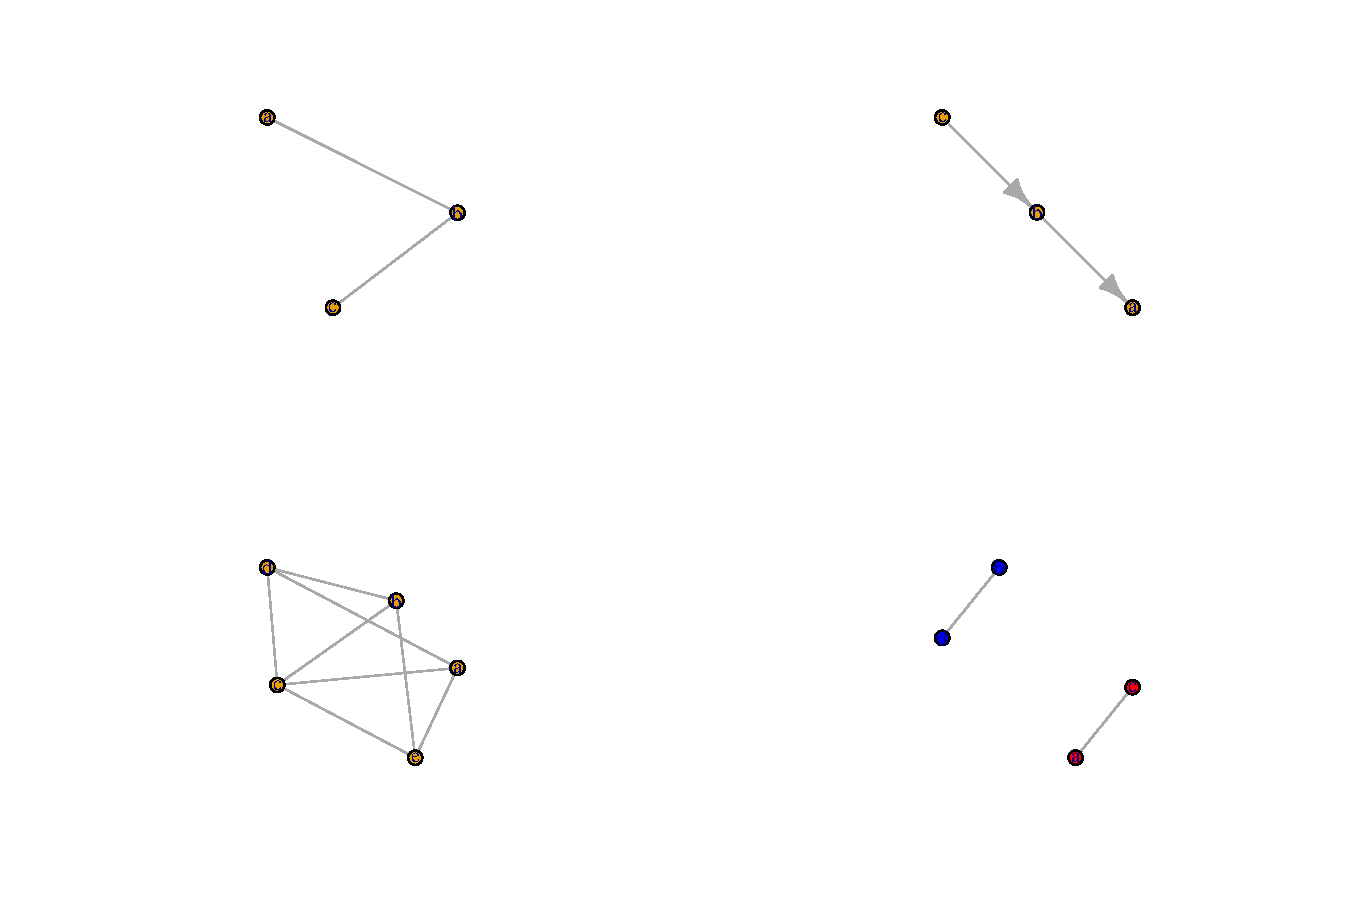
\includegraphics[width=.8\textwidth]{figures/basic_graphs-1} 

\end{knitrout}

\end{frame}

\begin{frame}
  \frametitle{Neighborhood, Degree}

  \begin{definition}[Neighborhood]
    The neighbors of a vertex are the nodes directly connected to this vertex:
    \[
      \clN(i) = \set{j\in\clV : (i,j) \in \clE}.
    \]
  \end{definition}
  
  \begin{definition}[Degree]
    The degree $d_i$ of a node $i$ is given by its number of neighbors, i.e. $|\clN(i)|$.
  \end{definition}

  \begin{block}{Remark}
    In digraphs, vertex degree is replaced by \alert{in-degree} and \alert{out-degree}.
  \end{block}

  \begin{proposition}
    In a graph $\clG = (\clV,\clE)$ the sum of the degree is given by $2|\clE|$. Hence \alert{this is always an even quantity}.
  \end{proposition}
  
  
\end{frame}

\begin{frame}
  \frametitle{Adjacency matrix and list of edges}

  \begin{definition}[Adjacency matrix]
    The connectivity of  $\clG = (\clV,\clE)$ is captured by the $|\clV|\times |\clV|$ matrix $\bA$:
    \[
      (\bA)_{ij} = \begin{cases}
      1  & \text{ if } i \sim j,\\
      0  & \text{otherwise}.
      \end{cases}
    \]
  \end{definition}

  \begin{proposition}
    The degree of $\clG$ are then simply obtained as the row-wise and/or column-wise sums of $\bA$.
  \end{proposition}

  \begin{block}{Remark}
    If the list of vertices is known, the only information which needs to be stored is the list of edges. In terms of storage, this is equivalent to a sparse matrix representation.
  \end{block}
  
\end{frame}

\begin{frame}
  \frametitle{Layout and Vizualization}
  
  \begin{itemize}
    \item Vizualization of large networks is a field of research in its own
    \item Be carefull with graphical interpretation of (large) networks
  \end{itemize}

\begin{knitrout}\scriptsize
\definecolor{shadecolor}{rgb}{0.969, 0.969, 0.969}\color{fgcolor}\begin{kframe}
\begin{alltt}
\hlkwd{library}\hlstd{(igraph)}

\hlkwd{library}\hlstd{(sand)}

\hlstd{GLattice} \hlkwb{<-} \hlkwd{graph.lattice}\hlstd{(}\hlkwd{c}\hlstd{(}\hlnum{5}\hlstd{,}\hlnum{5}\hlstd{,}\hlnum{5}\hlstd{))}

\hlstd{GBlog}    \hlkwb{<-} \hlstd{aidsblog}
\end{alltt}
\end{kframe}
\end{knitrout}
  
\end{frame}

\begin{frame}
  \frametitle{Layout and Vizualization}
  \framesubtitle{Example with circle plot}
  


\begin{knitrout}\scriptsize
\definecolor{shadecolor}{rgb}{0.969, 0.969, 0.969}\color{fgcolor}\begin{kframe}
\begin{alltt}
\hlkwd{par}\hlstd{(}\hlkwc{mfrow}\hlstd{=}\hlkwd{c}\hlstd{(}\hlnum{1}\hlstd{,}\hlnum{2}\hlstd{))}

\hlkwd{plot}\hlstd{(GLattice,} \hlkwc{layout}\hlstd{=layout.circle);} \hlkwd{title}\hlstd{(}\hlstr{"5x5x5 lattice"}\hlstd{)}

\hlkwd{plot}\hlstd{(GBlog   ,} \hlkwc{layout}\hlstd{=layout.circle);} \hlkwd{title}\hlstd{(}\hlstr{"blog network"}\hlstd{)}
\end{alltt}
\end{kframe}
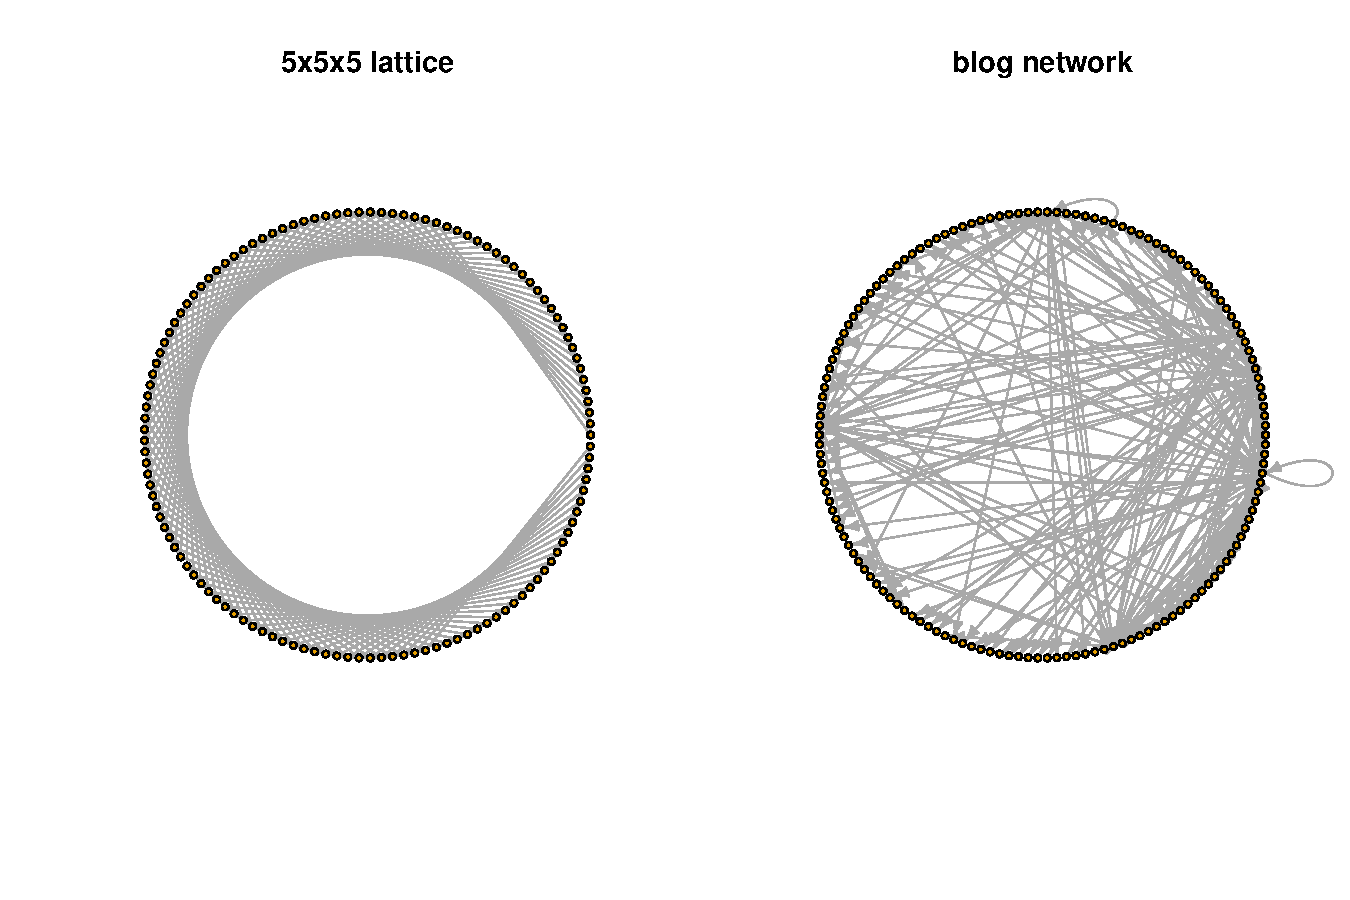
\includegraphics[width=.8\textwidth]{figures/vizu_3-1} 

\end{knitrout}
  
\end{frame}

\begin{frame}
  \frametitle{Layout and Vizualization}
  \framesubtitle{Example with Fruchterman and Reingold}

\begin{knitrout}\scriptsize
\definecolor{shadecolor}{rgb}{0.969, 0.969, 0.969}\color{fgcolor}\begin{kframe}
\begin{alltt}
\hlkwd{par}\hlstd{(}\hlkwc{mfrow}\hlstd{=}\hlkwd{c}\hlstd{(}\hlnum{1}\hlstd{,}\hlnum{2}\hlstd{))}

\hlkwd{plot}\hlstd{(GLattice,} \hlkwc{layout}\hlstd{=layout.fruchterman.reingold);} \hlkwd{title}\hlstd{(}\hlstr{"5x5x5 lattice"}\hlstd{)}

\hlkwd{plot}\hlstd{(GBlog   ,} \hlkwc{layout}\hlstd{=layout.fruchterman.reingold);} \hlkwd{title}\hlstd{(}\hlstr{"blog network"}\hlstd{)}
\end{alltt}
\end{kframe}
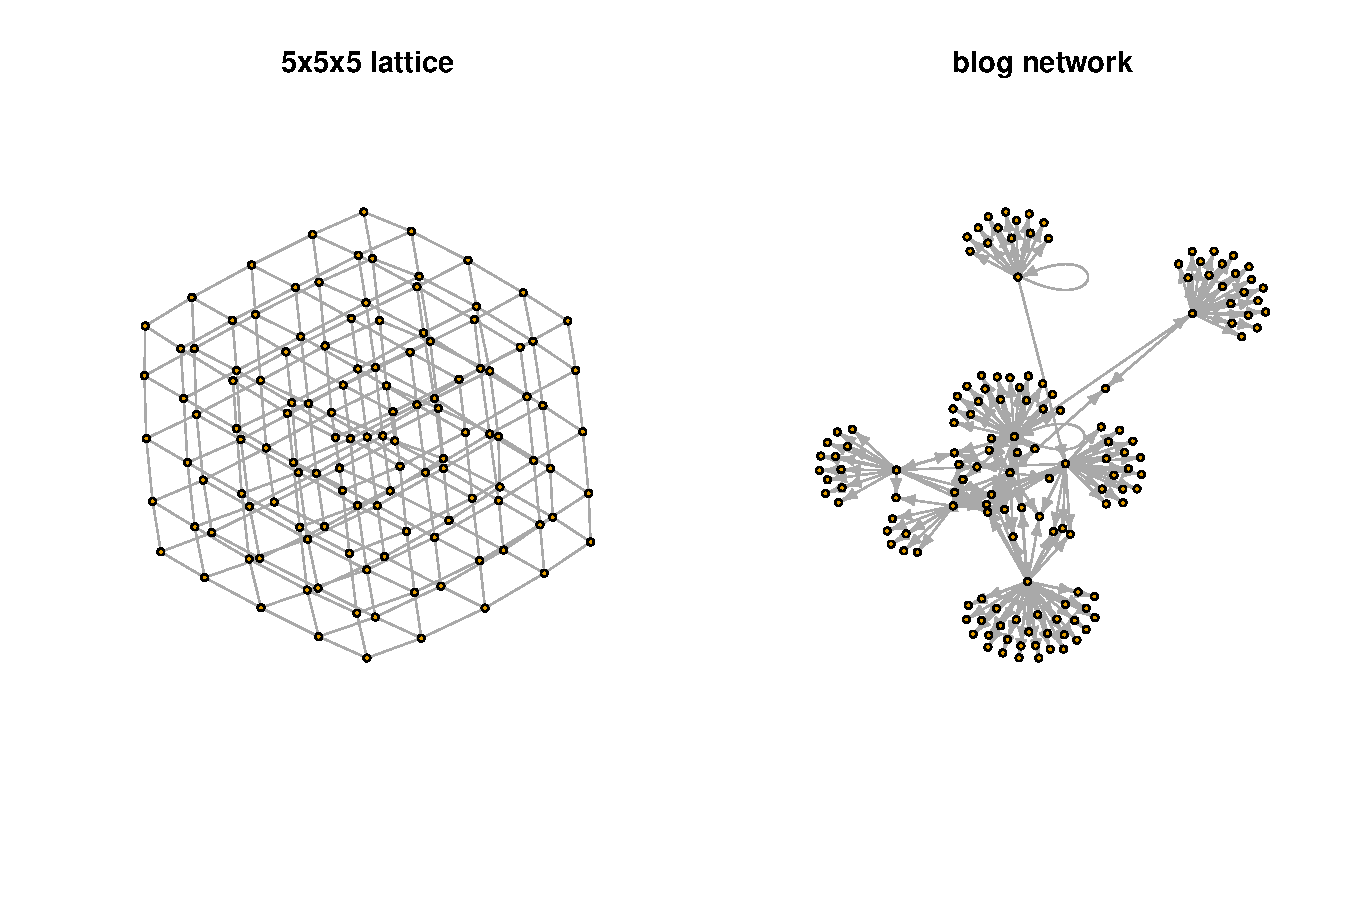
\includegraphics[width=.8\textwidth]{figures/vizu_4-1} 

\end{knitrout}
  
\end{frame}

\begin{frame}[fragile, allowframebreaks]
  \frametitle{Layout and Vizualization: \textbf{ggraph} way}
 
\begin{knitrout}\scriptsize
\definecolor{shadecolor}{rgb}{0.969, 0.969, 0.969}\color{fgcolor}\begin{kframe}
\begin{alltt}
\hlkwd{library}\hlstd{(ggraph)}
\hlkwd{library}\hlstd{(gridExtra)}
\hlstd{g1} \hlkwb{<-} \hlkwd{ggraph}\hlstd{(GBlog,} \hlkwc{layout} \hlstd{=} \hlstr{"fr"}\hlstd{)} \hlopt{+}
  \hlkwd{geom_edge_link}\hlstd{(}\hlkwc{color} \hlstd{=} \hlstr{"lightgray"}\hlstd{)} \hlopt{+} \hlkwd{geom_node_point}\hlstd{()} \hlopt{+} \hlkwd{theme_void}\hlstd{()}

\hlstd{g2} \hlkwb{<-} \hlkwd{ggraph}\hlstd{(GBlog   ,} \hlkwc{layout} \hlstd{=} \hlstr{"kk"}\hlstd{)} \hlopt{+}
  \hlkwd{geom_edge_link}\hlstd{(}\hlkwc{color} \hlstd{=} \hlstr{"lightgray"}\hlstd{)} \hlopt{+} \hlkwd{geom_node_point}\hlstd{()} \hlopt{+} \hlkwd{theme_void}\hlstd{()}

\hlstd{g3} \hlkwb{<-} \hlkwd{ggraph}\hlstd{(GBlog,} \hlkwc{layout} \hlstd{=} \hlstr{"linear"}\hlstd{)} \hlopt{+}
  \hlkwd{geom_edge_arc}\hlstd{(}\hlkwd{aes}\hlstd{(}\hlkwc{alpha}\hlstd{=..index..),} \hlkwc{show.legend} \hlstd{=} \hlnum{FALSE}\hlstd{)} \hlopt{+}
  \hlkwd{geom_node_point}\hlstd{()} \hlopt{+} \hlkwd{theme_void}\hlstd{()}

\hlstd{g4} \hlkwb{<-} \hlkwd{ggraph}\hlstd{(GBlog   ,} \hlkwc{layout} \hlstd{=} \hlstr{"linear"}\hlstd{,} \hlkwc{circular} \hlstd{=} \hlnum{TRUE}\hlstd{)} \hlopt{+}
  \hlkwd{geom_edge_link}\hlstd{(}\hlkwd{aes}\hlstd{(}\hlkwc{alpha}\hlstd{=..index..),} \hlkwc{show.legend} \hlstd{=} \hlnum{FALSE}\hlstd{)} \hlopt{+}
  \hlkwd{geom_node_point}\hlstd{()} \hlopt{+} \hlkwd{theme_void}\hlstd{()}

\hlkwd{grid.arrange}\hlstd{(g1, g2, g3, g4,} \hlkwc{nrow} \hlstd{=} \hlnum{2}\hlstd{,} \hlkwc{ncol} \hlstd{=} \hlnum{2}\hlstd{)}
\end{alltt}
\end{kframe}
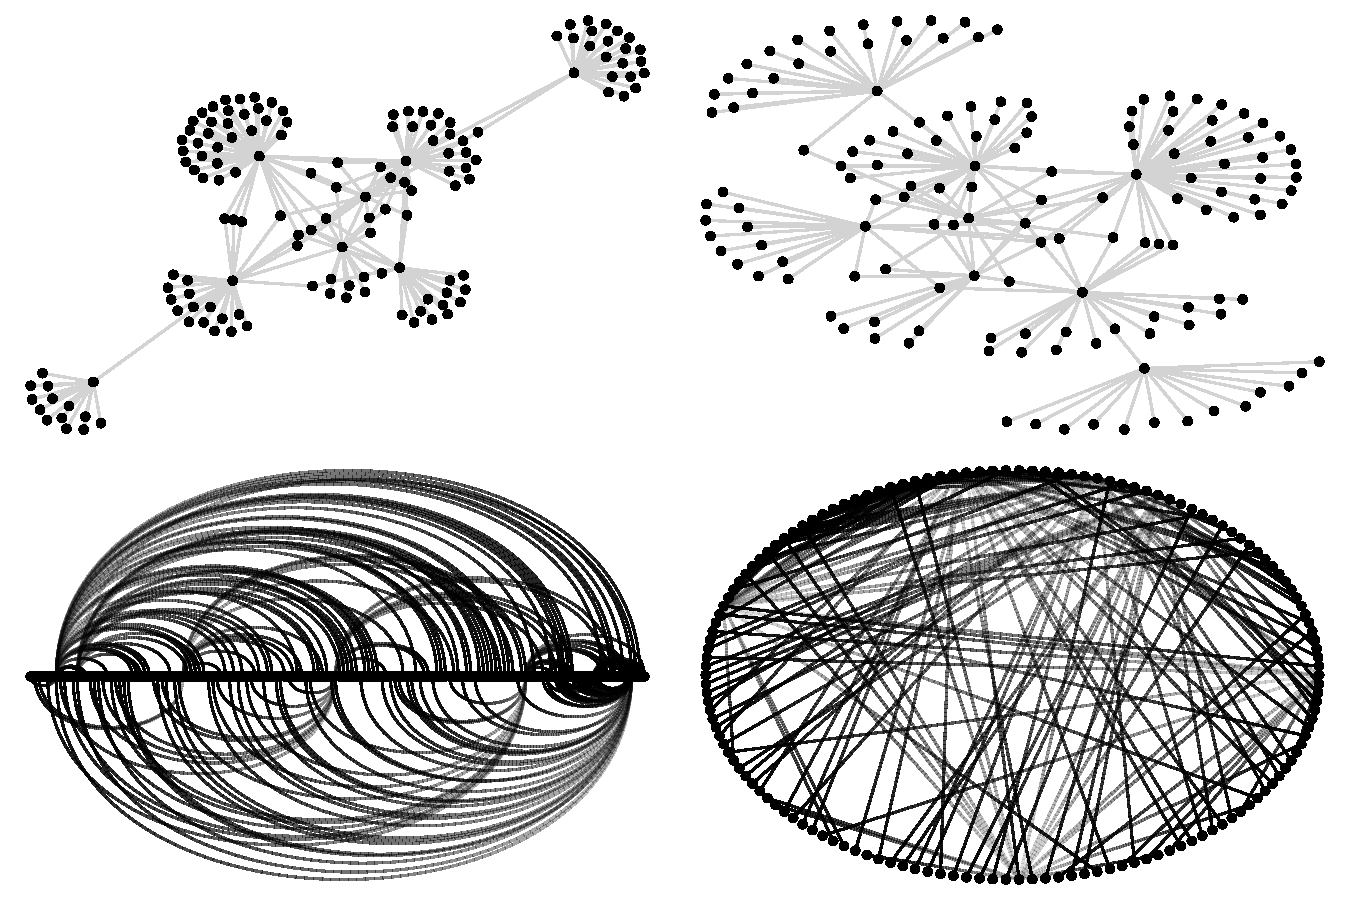
\includegraphics[width=.8\textwidth]{figures/ggraph_vizu_1-1} 

\end{knitrout}
\end{frame}

\begin{frame}
  \frametitle{Layout and Vizualization}
  \framesubtitle{Do not be fooled by the plot}

\begin{knitrout}\scriptsize
\definecolor{shadecolor}{rgb}{0.969, 0.969, 0.969}\color{fgcolor}\begin{kframe}
\begin{alltt}
\hlstd{g.tree} \hlkwb{<-} \hlkwd{graph.formula}\hlstd{(}\hlnum{1}\hlopt{-+}\hlnum{2}\hlstd{,}\hlnum{1}\hlopt{-+}\hlnum{3}\hlstd{,}\hlnum{1}\hlopt{-+}\hlnum{4}\hlstd{,}\hlnum{2}\hlopt{-+}\hlnum{5}\hlstd{,}\hlnum{2}\hlopt{-+}\hlnum{6}\hlstd{,}\hlnum{2}\hlopt{-+}\hlnum{7}\hlstd{,} \hlnum{3}\hlopt{-+}\hlnum{8}\hlstd{,}\hlnum{3}\hlopt{-+}\hlnum{9}\hlstd{,}\hlnum{4}\hlopt{-+}\hlnum{10}\hlstd{)}

\hlkwd{par}\hlstd{(}\hlkwc{mfrow}\hlstd{=}\hlkwd{c}\hlstd{(}\hlnum{1}\hlstd{,} \hlnum{3}\hlstd{))}

\hlkwd{igraph.options}\hlstd{(}\hlkwc{vertex.size}\hlstd{=}\hlnum{30}\hlstd{,} \hlkwc{edge.arrow.size}\hlstd{=}\hlnum{0.5}\hlstd{,} \hlkwc{vertex.label}\hlstd{=}\hlkwa{NULL}\hlstd{)}

\hlkwd{plot}\hlstd{(g.tree,} \hlkwc{layout}\hlstd{=layout.circle)}

\hlkwd{plot}\hlstd{(g.tree,} \hlkwc{layout}\hlstd{=}\hlkwd{layout.reingold.tilford}\hlstd{(g.tree,}  \hlkwc{circular}\hlstd{=T))}

\hlkwd{plot}\hlstd{(g.tree,} \hlkwc{layout}\hlstd{=layout.reingold.tilford)}
\end{alltt}
\end{kframe}
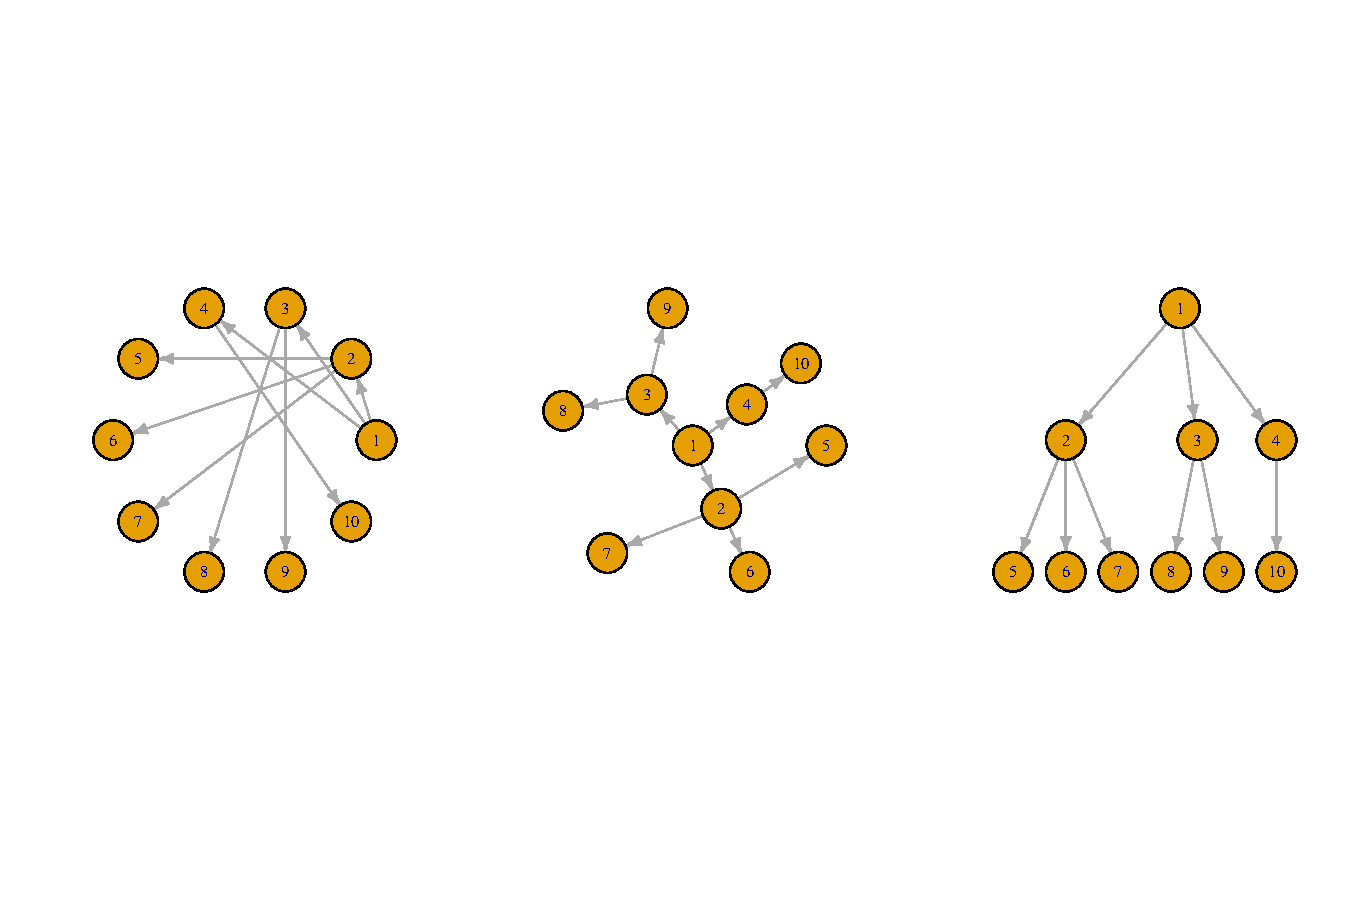
\includegraphics[width=.8\textwidth]{figures/vizu_5-1} 

\end{knitrout}
  
\end{frame}


%% ==========================================================================
\section{Descriptive statistics}
%% ==========================================================================

%% ==========================================================================
\subsection{Vertex characteristics}

\begin{frame}
  \frametitle{Vertex degree}
  
  \begin{definition}[Degree distribution]
    In a graph $\clG = (\clV, \clE)$, recall that $d_i$ counts the number of incident edges in $\clE$ to $i$. Define $f_d$ to be
    the fraction of vertices $i\in \clV$ with degree $d_i=d$. The collection $\set{f_d, d\geq 0}$ is called the \alert{degree distribution} of $\clG$.
  \end{definition}
  
  \begin{block}{Property}
    Many real world networks have a degree distribution fitting well power law distributions: 
    \[
      f_{d_i}(d) = \P(d_i = d) = \frac{c}{d^\gamma}, \quad c\in\Rset, \gamma > 0.
    \]
  \end{block}
  Those heavy-tail distributions describe few vertices with very high degrees.
\end{frame}

\begin{frame}
  \frametitle{Vertex degree: example I}

\begin{knitrout}\scriptsize
\definecolor{shadecolor}{rgb}{0.969, 0.969, 0.969}\color{fgcolor}\begin{kframe}
\begin{alltt}
\hlkwd{library}\hlstd{(sand)}
\hlkwd{data}\hlstd{(karate)}

\hlkwd{par}\hlstd{(}\hlkwc{mfrow}\hlstd{=}\hlkwd{c}\hlstd{(}\hlnum{1}\hlstd{,}\hlnum{2}\hlstd{))}
\hlkwd{plot}\hlstd{(karate)}

\hlkwd{hist}\hlstd{(}\hlkwd{degree}\hlstd{(karate),} \hlkwc{col}\hlstd{=}\hlkwd{adjustcolor}\hlstd{(}\hlstr{"lightblue"}\hlstd{,} \hlkwc{alpha.f} \hlstd{=} \hlnum{0.5}\hlstd{),} \hlkwc{main}\hlstd{=}\hlstr{""}\hlstd{)}
\end{alltt}
\end{kframe}
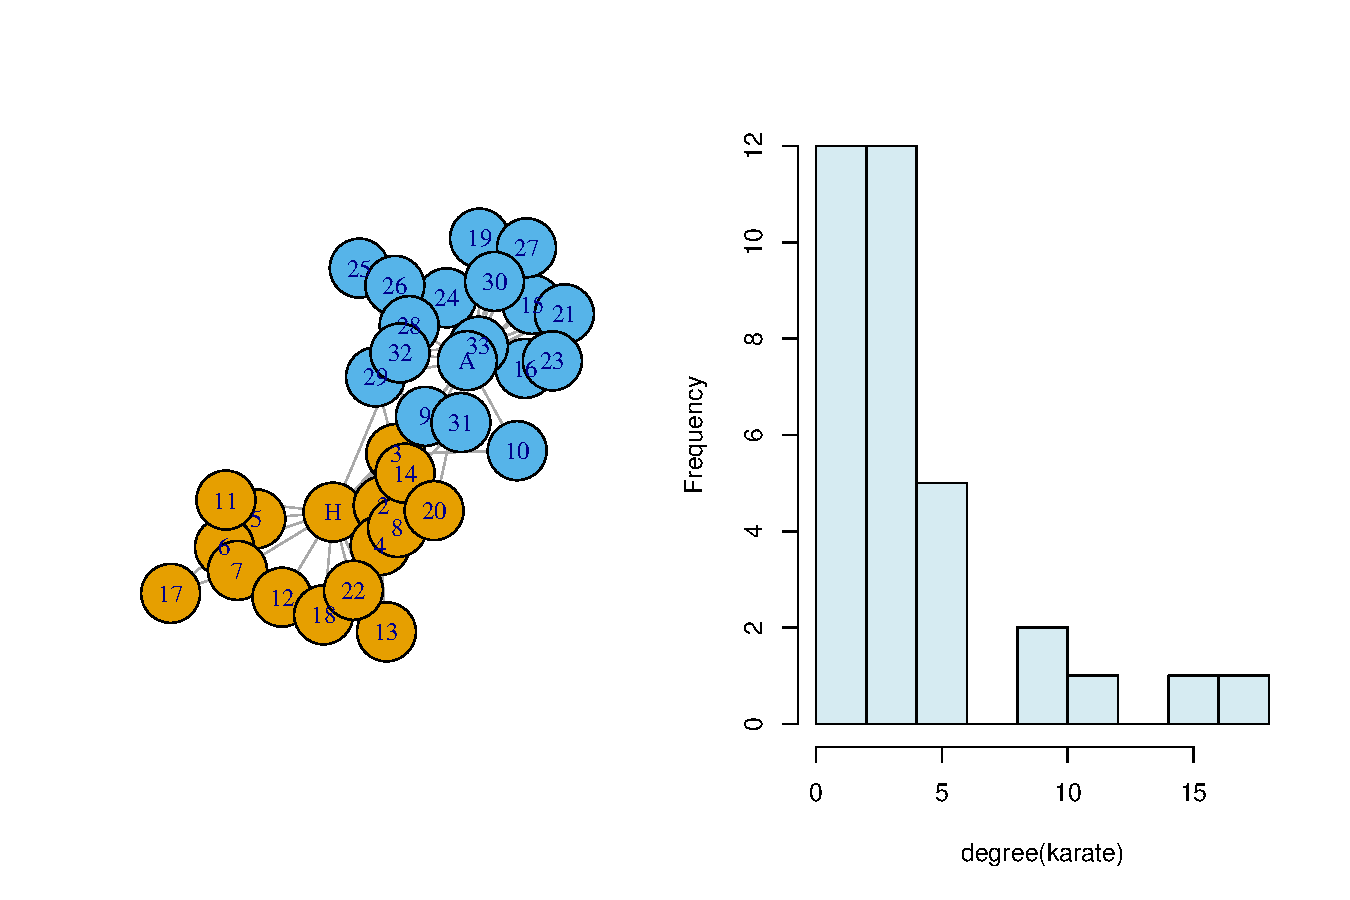
\includegraphics[width=.8\textwidth]{figures/degree_1-1} 

\end{knitrout}
      
\end{frame}

\begin{frame}
  \frametitle{Vertex degree: example II}

\begin{knitrout}\scriptsize
\definecolor{shadecolor}{rgb}{0.969, 0.969, 0.969}\color{fgcolor}\begin{kframe}
\begin{alltt}
\hlkwd{library}\hlstd{(igraphdata)}
\hlkwd{data}\hlstd{(yeast)}

\hlstd{degrees.yeast} \hlkwb{<-} \hlkwd{rev}\hlstd{(}\hlkwd{sort}\hlstd{(}\hlkwd{degree.distribution}\hlstd{(yeast)))}

\hlkwd{plot}\hlstd{(degrees.yeast[degrees.yeast}\hlopt{!=}\hlnum{0}\hlstd{],} \hlkwc{log}\hlstd{=}\hlstr{"xy"}\hlstd{,} \hlkwc{col}\hlstd{=}\hlkwd{adjustcolor}\hlstd{(}\hlstr{"blue"}\hlstd{,} \hlkwc{alpha.f} \hlstd{=} \hlnum{0.5}\hlstd{),} \hlkwc{pch}\hlstd{=}\hlnum{16}\hlstd{,} \hlkwc{xlab}\hlstd{=}\hlstr{"log degree"}\hlstd{,} \hlkwc{ylab}\hlstd{=}\hlstr{"log-intensity"}\hlstd{)}
\end{alltt}
\end{kframe}
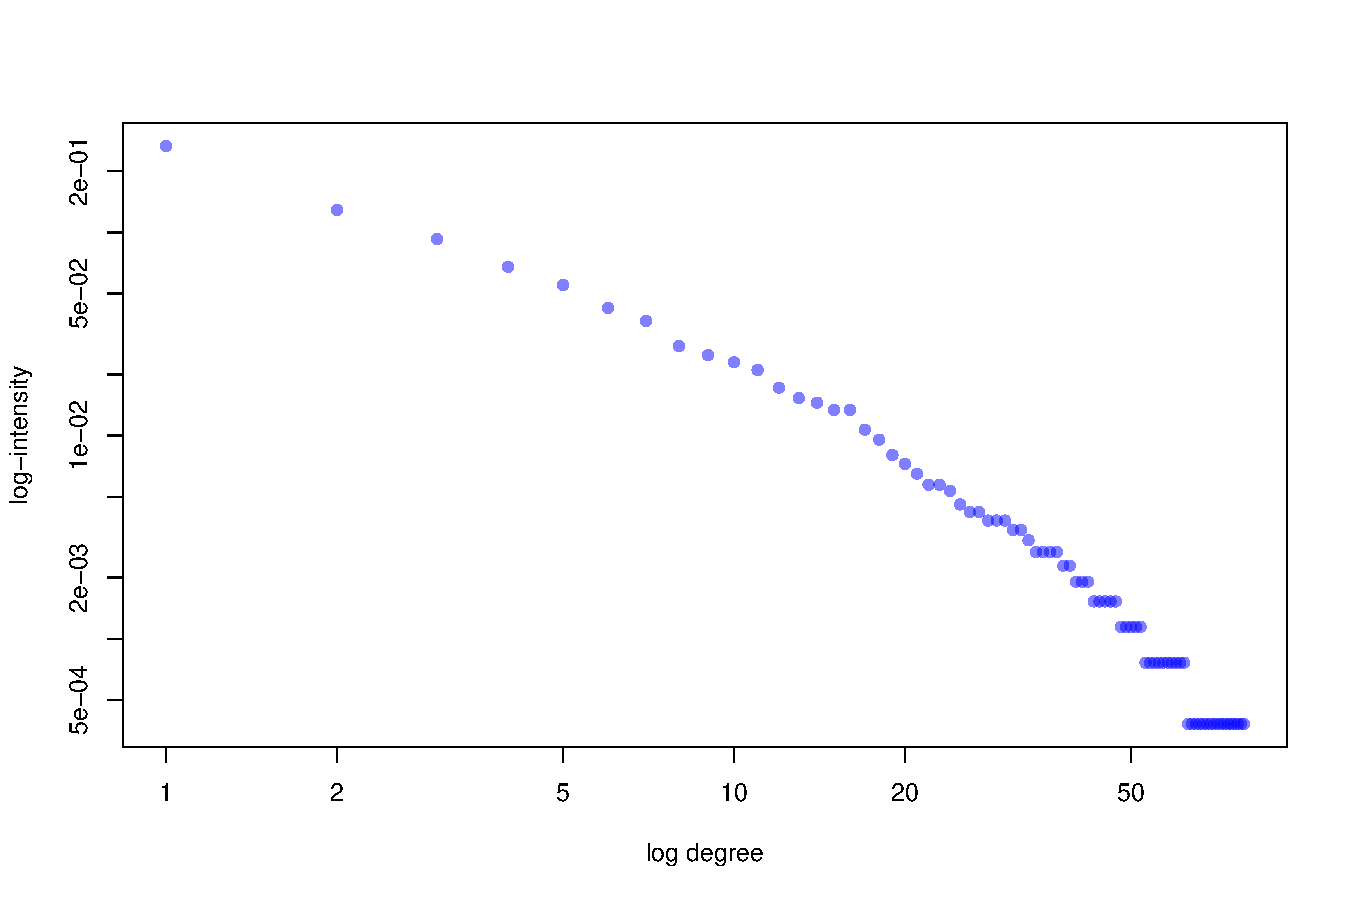
\includegraphics[width=.8\textwidth]{figures/degree_2-1} 

\end{knitrout}
      
\end{frame}

\begin{frame}[allowframebreaks]
  \frametitle{Distance and diameter}

  \begin{definition}[distance]
    \begin{itemize}
    \item \alert{The Length}  of a path $e_1,\dots, e_k$ is the number of edges enterin the path (here $k$).
    \item If two nodes $i,j$ are connected in $G$, then \alert{the distance} $\ell_{ij}$ is the length of the shortest path between $i$ and $j$. If the two nodes are not connected then $\ell_{ij} = \infty$.
    \end{itemize}
  \end{definition}

  \begin{definition}[diameter]
    The diameter of $\clG$ is the greatest distance between two nodes:
    \[
      \mathrm{diameter(\clG)} = \max_{(i,j)\in\clV\times\clV} \left(\ell_{ij}\right)
    \]
  \end{definition}

\end{frame}

\begin{frame}[fragile,allowframebreaks]
  \frametitle{Distance, Diameter: example}
\begin{knitrout}\scriptsize
\definecolor{shadecolor}{rgb}{0.969, 0.969, 0.969}\color{fgcolor}\begin{kframe}
\begin{alltt}
\hlkwd{library}\hlstd{(Matrix)}
\hlkwd{data}\hlstd{(ppi.CC)}
\hlkwd{diameter}\hlstd{(ppi.CC)}
\end{alltt}
\begin{verbatim}
## [1] 12
\end{verbatim}
\begin{alltt}
\hlkwd{average.path.length}\hlstd{(ppi.CC)}
\end{alltt}
\begin{verbatim}
## [1] 4.448039
\end{verbatim}
\begin{alltt}
\hlkwd{image}\hlstd{(}\hlkwd{Matrix}\hlstd{(}\hlkwd{distances}\hlstd{(ppi.CC)))}
\end{alltt}
\end{kframe}
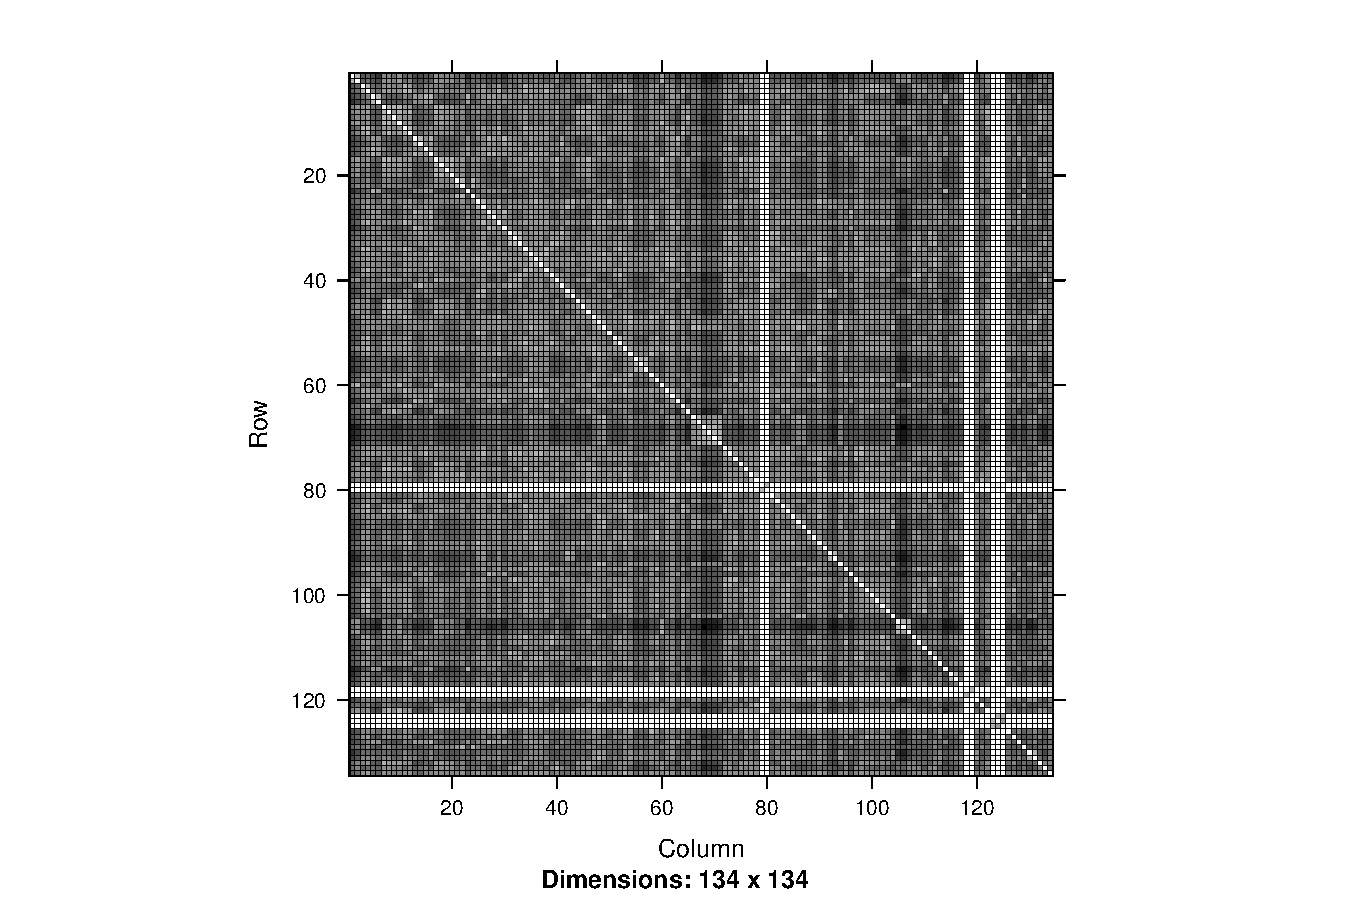
\includegraphics[width=.8\textwidth]{figures/distances1-1} 

\end{knitrout}
\end{frame}

\begin{frame}
  \frametitle{Vertex centrality: closeness}

  \begin{block}{Question}
    How important is the node/vertice in the network?
  \end{block}

  \begin{definition}[Farness, Closeness]
    Farness is the sum of the length of the shortest paths between the node and all other nodes in the graph. Closeness is defined as its reciprocal:
    \[C(x)={\frac  {1}{\sum _{y}d(y,x)}}.\]
    $\rightsquigarrow$ \textit{The more central a node is, the closer it is to all other nodes.}
  \end{definition}

\end{frame}

\begin{frame}
  \frametitle{Vertex centrality: betweenness}

  \begin{block}{Question}
    How important is the node/vertice in the network?
  \end{block}

  \begin{definition}[Betweenness]
    For every pairs of vertices, there exists at least one shortest path between the vertices such that the number of edges that the path passes through is minimized.
    The betweenness centrality for each vertex is the number of these shortest paths that pass through the vertex: 
    \[
        g(i)=\sum _{{j\neq i\neq k}}{\frac  {\sigma _{{jk}}(i)}{\sigma _{{jk}}}}    
    \]
    where $\sigma _{jk}$ is the total number of shortest paths from node $j$ to node $k$ and $\sigma _{jk}(i)$ the number of those paths that pass through $i$.

  \end{definition}

\end{frame}

\begin{frame}[fragile]
  \frametitle{Example for karate club data set}
  \framesubtitle{administrator and instructor are in blue and yellow}

\begin{knitrout}\scriptsize
\definecolor{shadecolor}{rgb}{0.969, 0.969, 0.969}\color{fgcolor}
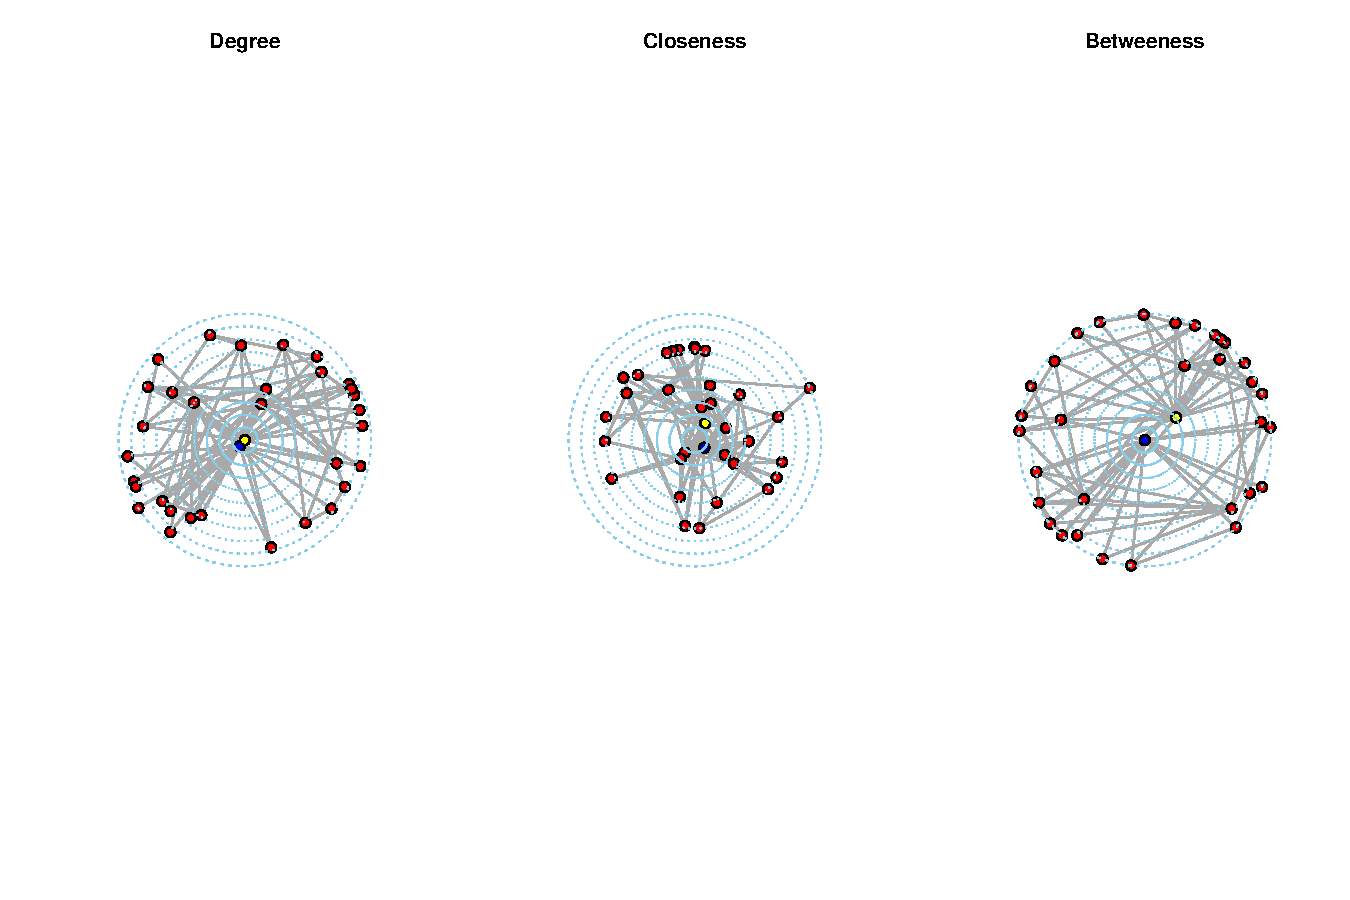
\includegraphics[width=\textwidth]{figures/density-1} 

\end{knitrout}



\end{frame}

\begin{frame}
  \frametitle{Jaccard Coefficient}

  \begin{definition}[Jaccard Coefficient or Jaccard Index]
The Jaccard coefficient \alert{measures similarity between finite sample sets}, and is defined as the size of the intersection divided by the size of the union of the sample sets:
  \[
  J(A,B)=\frac{|A\cap B|}{|A\cup B|} =\frac{|A\cap B|}{|A|+|B|-|A\cap B|}.
  \]
  \end{definition}

  \begin{block}{Example}
  It can be used to compared two sets of egdes. For instance
  \begin{itemize}
    \item for two networks $\clG$ and $\clH$ defined on the same set of node, we can compare the sets $\clE_\clG$ and $\clE_\clH$.
    \item for a networks $\clG$ we can compute similarity between nodes with the Jaccard index and use it to define a weighted graph of similarity.
  \end{itemize}
  \end{block}

\end{frame}

\begin{frame}[fragile]
  \frametitle{Jaccard Coefficient: example}

Plot the yeast PPI interaction network
\begin{knitrout}\scriptsize
\definecolor{shadecolor}{rgb}{0.969, 0.969, 0.969}\color{fgcolor}\begin{kframe}
\begin{alltt}
\hlkwd{library}\hlstd{(sand)}
\hlkwd{library}\hlstd{(igraph)}
\hlkwd{plot}\hlstd{(ppi.CC,} \hlkwc{vertex.size}\hlstd{=}\hlnum{6}\hlstd{,} \hlkwc{vertex.label}\hlstd{=}\hlnum{NA}\hlstd{,} \hlkwc{layout}\hlstd{=layout_in_circle)}
\end{alltt}
\end{kframe}
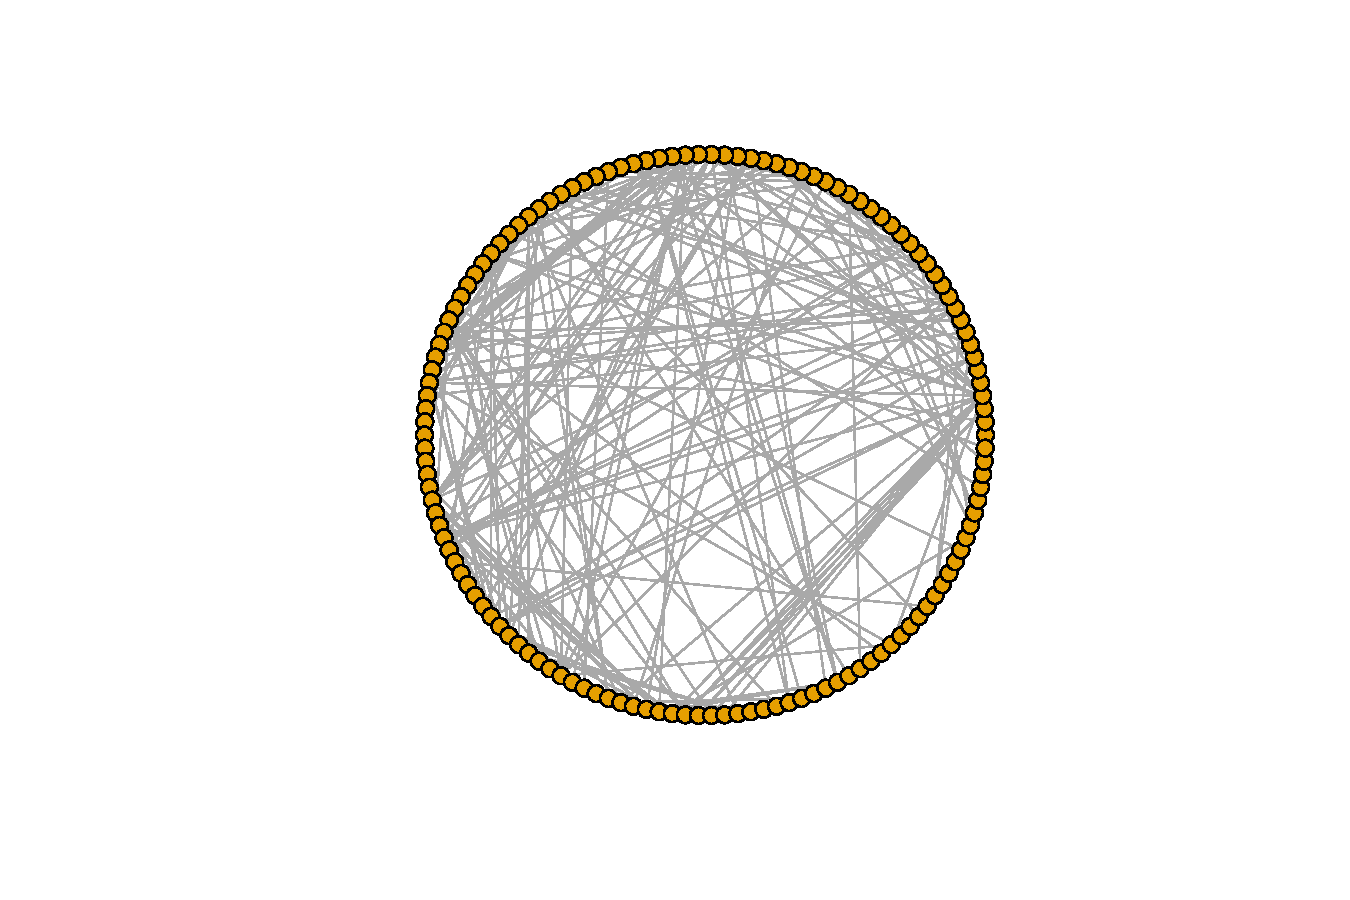
\includegraphics[width=.8\textwidth]{figures/jaccard-1} 

\end{knitrout}

\end{frame}

\begin{frame}[fragile]
  \frametitle{Jaccard Coefficient: example II}

Compute Jaccard similarity between vertices and give a image of this
\begin{knitrout}\scriptsize
\definecolor{shadecolor}{rgb}{0.969, 0.969, 0.969}\color{fgcolor}\begin{kframe}
\begin{alltt}
\hlkwd{library}\hlstd{(Matrix)}
\hlkwd{image}\hlstd{(}\hlkwd{Matrix}\hlstd{(igraph}\hlopt{::}\hlkwd{similarity}\hlstd{(ppi.CC,} \hlkwc{method} \hlstd{=} \hlstr{"jaccard"}\hlstd{)))}
\end{alltt}
\end{kframe}
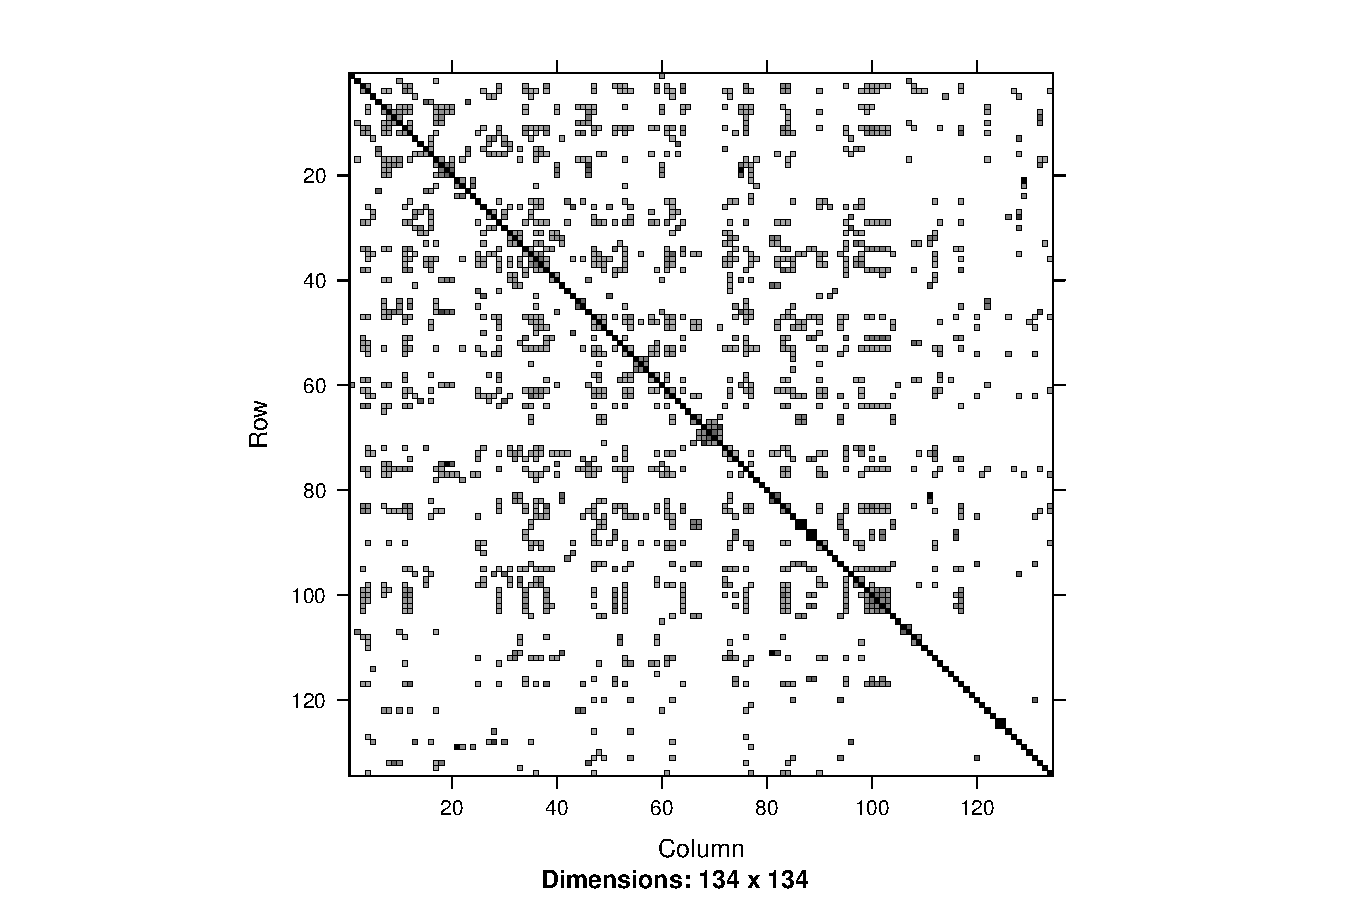
\includegraphics[width=.8\textwidth]{figures/jaccardplot-1} 

\end{knitrout}

\end{frame}

%% ==========================================================================
\subsection{Local measurements}

\begin{frame}
  \frametitle{Density}

  \begin{block}{Question}
    Is the network locally \alert{dense} in some sense?
  \end{block}

  \begin{definition}[Clique]
    In an undirected graph, a clique is a subset of the vertices such that \alert{every two distinct vertices are adjacent}.
  \end{definition}


  \begin{definition}[Density]
    The density of a (sub)-graph $\clG = (\clV,\clE)$ is defined by
    \[
      \mathrm{density}(\clG) = \frac{2|\clE|}{|\clV|(|\clV| - 1)} = \frac{\bar{D}}{|V|-1},
    \]
    where $\bar{D}$ is the mean degree of the network: how much $\clG$ is close to a clique? 
  \end{definition}

\end{frame}

\begin{frame}
  \frametitle{Clustering}

  \begin{block}{Question}
    Is the network locally \alert{dense} in some sense?
  \end{block}

  \begin{definition}[Triangle]
    Triplets of vertices in the graph that are connected through a triangle. They correspond to transitive relationships. We let 
    \begin{itemize}
      \item $\tau_{\Delta}(i)$ be the number of triangles in $\clG$ where $i$ falls.
      \item $\tau_{3}(i)$ be the number of triplets in $\clG$ where $i$ falls.
    \end{itemize}    
  \end{definition}


  \begin{definition}[Clustering coefficient]
    \[
      \mathrm{clustering}(\clG) = \frac{1}{\clV_2} \sum_{i\in\clV_2} \tau_{\Delta}(i) / \tau_3(i),
    \]
    where $\clV_2$ is the set of vertices whose degree is greater or equal to 2.
  \end{definition}

\end{frame}

\begin{frame}
  \frametitle{Transitivity}

  \begin{block}{Question}
    Is the network locally \alert{dense} in some sense?
  \end{block}

  \begin{definition}[Triangle]
    Triplet of vertices in the graph that are connected through a triangle. They correspond to transitive relationships. We let 
    \begin{itemize}
      \item $\tau_{\Delta}(i)$ be the number of triangle in $\clG$ where $i$ falls.
      \item $\tau_{3}(i)$ be the number of triplet in $\clG$ where $i$ falls.
    \end{itemize}    
  \end{definition}

  \begin{definition}[Transitivity]
    
    \[
      \mathrm{transitivity}(\clG) = \frac{\sum_{\clV}\tau_{\Delta}(i)}{\sum_{\clV}\tau_3(i)},
    \]
  \end{definition}

\end{frame}

\begin{frame}[fragile]
  \frametitle{Local density: example}



Create ego graphs around teacher and instructor
\begin{knitrout}\scriptsize
\definecolor{shadecolor}{rgb}{0.969, 0.969, 0.969}\color{fgcolor}\begin{kframe}
\begin{alltt}
\hlkwd{data}\hlstd{(karate)}
\hlstd{ego.instr} \hlkwb{<-} \hlstd{igraph}\hlopt{::}\hlkwd{induced_subgraph}\hlstd{(karate,} \hlkwd{neighborhood}\hlstd{(karate,} \hlnum{1}\hlstd{,} \hlnum{1}\hlstd{)[[}\hlnum{1}\hlstd{]])}
\hlstd{ego.admin} \hlkwb{<-} \hlstd{igraph}\hlopt{::}\hlkwd{induced_subgraph}\hlstd{(karate,} \hlkwd{neighborhood}\hlstd{(karate,} \hlnum{1}\hlstd{,} \hlnum{34}\hlstd{)[[}\hlnum{1}\hlstd{]])}
\end{alltt}
\end{kframe}
\end{knitrout}

\begin{knitrout}\scriptsize
\definecolor{shadecolor}{rgb}{0.969, 0.969, 0.969}\color{fgcolor}
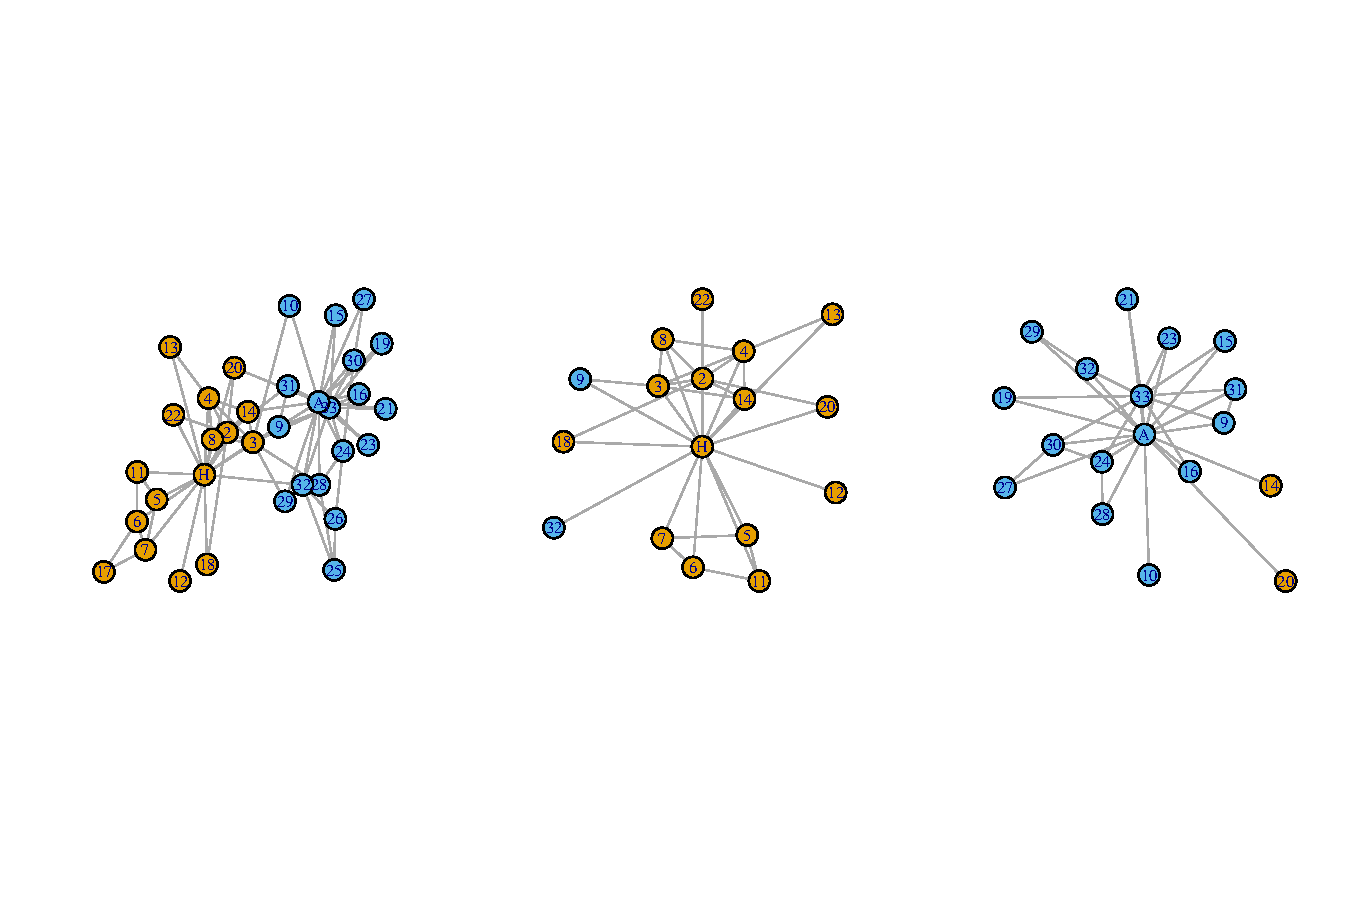
\includegraphics[width=.8\textwidth]{figures/density3-1} 

\end{knitrout}

\end{frame}

\begin{frame}[fragile]
  \frametitle{Local density: example (II)}

Look for graph density and transitivity/clustering either globally or locally
\begin{knitrout}\scriptsize
\definecolor{shadecolor}{rgb}{0.969, 0.969, 0.969}\color{fgcolor}\begin{kframe}
\begin{alltt}
\hlkwd{graph.density}\hlstd{(karate)}
\end{alltt}
\begin{verbatim}
## [1] 0.1390374
\end{verbatim}
\begin{alltt}
\hlkwd{graph.density}\hlstd{(ego.instr)}
\end{alltt}
\begin{verbatim}
## [1] 0.25
\end{verbatim}
\begin{alltt}
\hlkwd{graph.density}\hlstd{(ego.admin)}
\end{alltt}
\begin{verbatim}
## [1] 0.2091503
\end{verbatim}
\begin{alltt}
\hlkwd{transitivity}\hlstd{(karate)}
\end{alltt}
\begin{verbatim}
## [1] 0.2556818
\end{verbatim}
\begin{alltt}
\hlkwd{transitivity}\hlstd{(karate,} \hlstr{"local"}\hlstd{,} \hlkwc{vids} \hlstd{=} \hlkwd{c}\hlstd{(}\hlnum{1}\hlstd{,}\hlnum{34}\hlstd{))}
\end{alltt}
\begin{verbatim}
## [1] 0.1500000 0.1102941
\end{verbatim}
\end{kframe}
\end{knitrout}

\end{frame}


%% ==========================================================================
\section{Graph Partionning}
%% ==========================================================================

\begin{frame}
  \frametitle{Principle of graph partionning}

  \begin{definition}[Partition]
    A decomposition $\mathcal{C} = \{C_1,\dots,C_K\}$ of the vertices $\clV$ such that
    \begin{itemize}
      \item $C_k \cap C_{k'} = \emptyset$ for any $k\neq k'$
      \item $\bigcup_{k} C_k = \clV$
    \end{itemize}
  \end{definition}

  \vfill

  \begin{block}{Goal of graph paritionning}
    Form a partition of the vertices with unsupervized approach where the $\mathcal{C}$ is composed by \alert{"cohesive"} sets of vertices, for instance,
    \begin{enumerate}
      \item vertices well connected among themselves
      \item well separated from the remaining vertices
    \end{enumerate}
    
  \end{block}

\end{frame}

%% ==========================================================================
\subsection{Hierarchical clustering}

\begin{frame}
  \frametitle{Principle}
  \framesubtitle{}

  \begin{algorithm}[H]
    \KwIn{$n$ individuals with $p$ attributes)}
    \BlankLine\BlankLine
    \DontPrintSemicolon
      1. Compute the dissimilarity between groups \;
      2. Regroup the two most similar elements \;
      
      Iterate until all element are in a single group \;
    \BlankLine\BlankLine
    \KwOut{$n$ nested partitions from $\set{\set{1},\dots,\set{n}}$ to $\set{\set{1,\dots,n}}$}

    \caption{Agglomerative hierarchical clustering}
  \end{algorithm}
  
  \begin{block}{Ingredients}
    \begin{enumerate}
      \item a dissimilarity measure between singleton
      \item a distance measure between sets
    \end{enumerate}
  \end{block}

\end{frame}

\begin{frame}
  \frametitle{Dissimilarity measures}

  \begin{block}{Standards}
    Use standard distances on adjacency matrix:
    \begin{itemize}
      \item Euclidean distance: $\displaystyle x_{ij} = \sqrt{\sum_{ij} (A_{ik} - A_{jk})^2} $
      \item Manhattan distance: $\displaystyle x_{ij} = \sum_{ij} |A_{ik} - A_{jk})| $
      \item  etc\dots
    \end{itemize}  
  \end{block}

  \vfill

  \begin{block}{Graph-specific}
    For instance,  modularity, betweeness, etc.
  \end{block}
  
\end{frame}

\begin{frame}[fragile,allowframebreaks]
  \frametitle{Examples of graph clustering}

\begin{knitrout}\scriptsize
\definecolor{shadecolor}{rgb}{0.969, 0.969, 0.969}\color{fgcolor}\begin{kframe}
\begin{alltt}
\hlstd{hc} \hlkwb{<-} \hlkwd{cluster_fast_greedy}\hlstd{(karate)}
\hlkwd{plot}\hlstd{(hc,karate)}
\end{alltt}
\end{kframe}
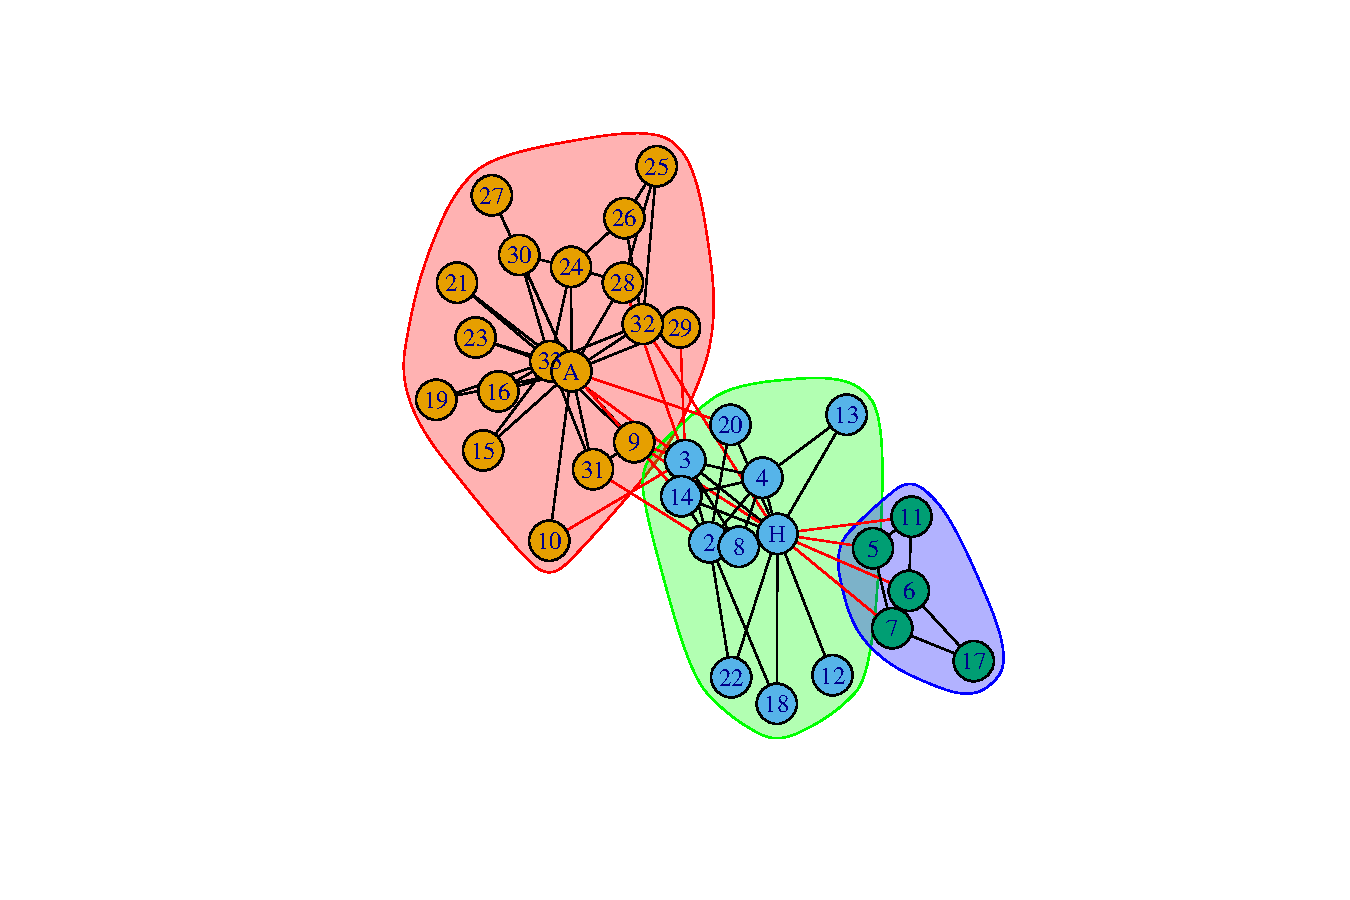
\includegraphics[width=.8\textwidth]{figures/unnamed-chunk-3-1} 

\end{knitrout}

\begin{knitrout}\scriptsize
\definecolor{shadecolor}{rgb}{0.969, 0.969, 0.969}\color{fgcolor}\begin{kframe}
\begin{alltt}
\hlstd{hc} \hlkwb{<-} \hlkwd{cluster_edge_betweenness}\hlstd{(karate)}
\hlkwd{plot}\hlstd{(hc,karate)}
\end{alltt}
\end{kframe}
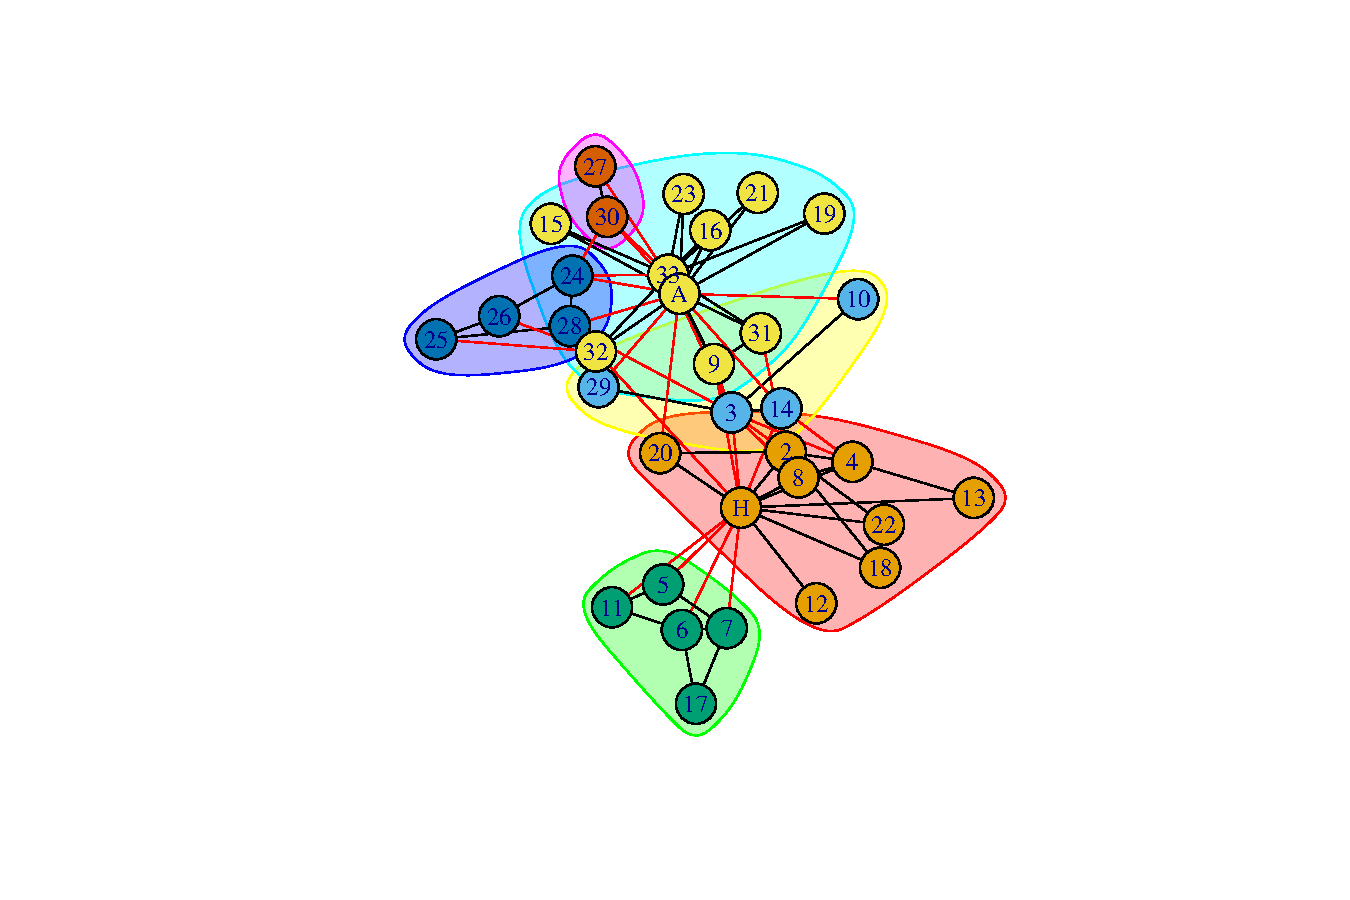
\includegraphics[width=.8\textwidth]{figures/unnamed-chunk-4-1} 

\end{knitrout}

\begin{knitrout}\scriptsize
\definecolor{shadecolor}{rgb}{0.969, 0.969, 0.969}\color{fgcolor}\begin{kframe}
\begin{alltt}
\hlstd{hc} \hlkwb{<-} \hlkwd{cluster_walktrap}\hlstd{(karate)}
\hlkwd{plot}\hlstd{(hc,karate)}
\end{alltt}
\end{kframe}
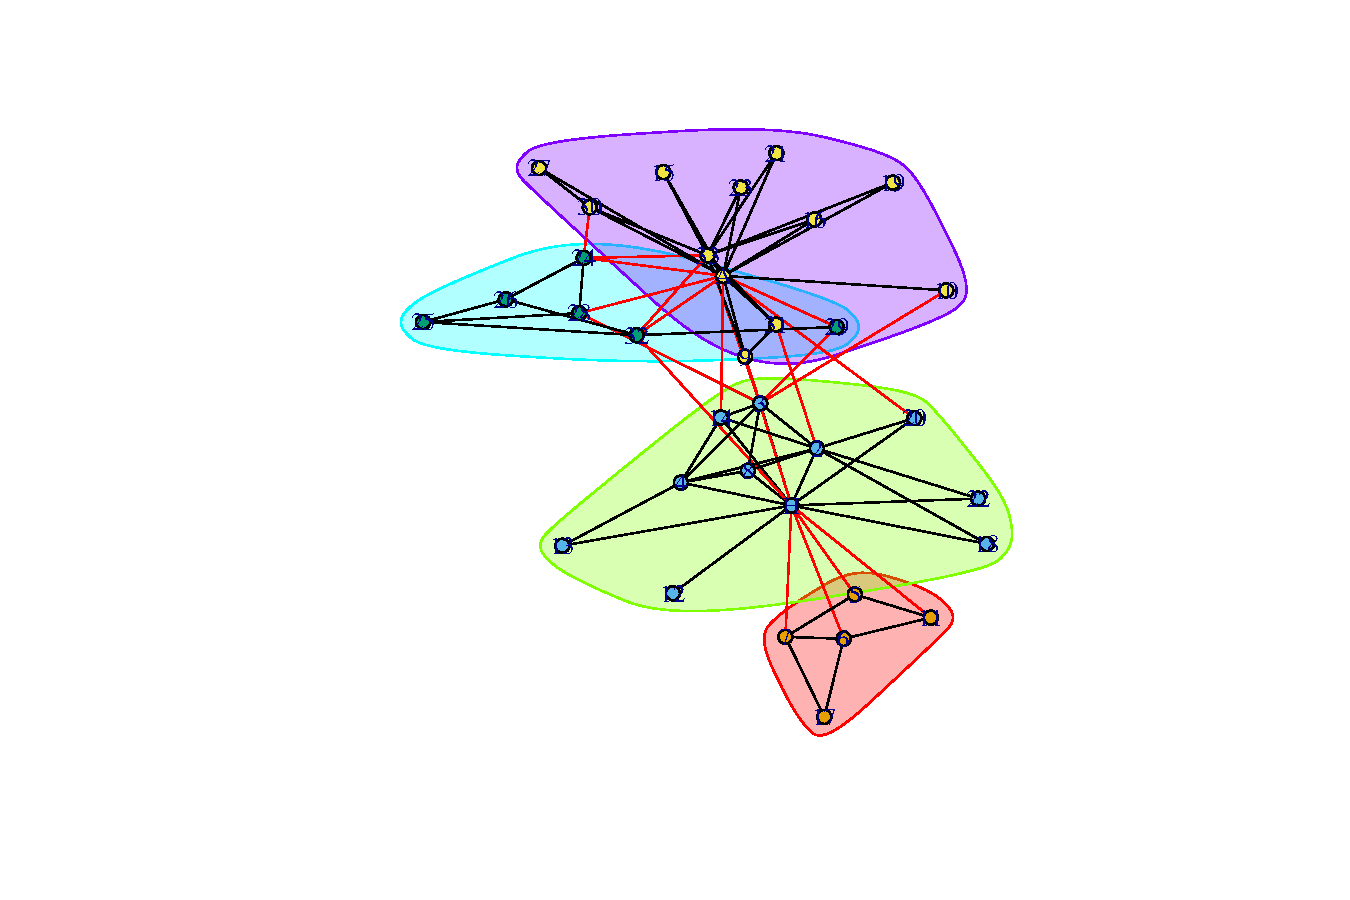
\includegraphics[width=.8\textwidth]{figures/unnamed-chunk-5-1} 

\end{knitrout}

\end{frame}

%% ==========================================================================
\subsection{Spectral Clustering}

\begin{frame}
  \frametitle{Graph Laplacian}

  \begin{definition}[(Un-normalized) Laplacian]
    The Laplacian matrix $\bL$, resulting from the modified incidence matrix $\tilde\bB$ $\tilde{\! B}_{ij}= 1/-1$ if $i$ is incident to $j$ as tail/head, is defined by 
    \[
      \bL = \tilde \bB \tilde \bB^\intercal = \bD - \bA,
    \]
    where $\bD = \diag(d_i, i\in\clV)$ is the diagonal matrix of degrees. 
  \end{definition}

  \begin{block}{Remark}
    \begin{itemize}
    \item $\bL$ is called Laplacian by analogy to the second order derivative (see below).
    \item Spectrum of $\bL$ has much to say about the structure of the graph $\clG$.
    \end{itemize}
  \end{block}

\end{frame}

\begin{frame}
  \frametitle{Spectral Clustering}
    
  \begin{block}{Principle}
  
  \begin{enumerate}
    \item Use the spectral property of $\bL$ to perform clustering in the eigen space \medskip
    \item If the network have $K$ connected components, the first $K$ eigenvectors are $\mathbf{1}$ span the eigenspace associated with eigenvalue $0$ \medskip
    \item Applying a simple clustering algorithm to the rows of the $K$ first eigenvectors separate the components
  \end{enumerate}
  $\rightsquigarrow$ This principle generalizes to a graph with a single component: spectral clustering tends to separates groups of nodes which are highly connected together
  
  \end{block}
  
\end{frame}

\begin{frame}[fragile]
  \frametitle{Clustering based on the first non null eigenvalue}
  
\begin{knitrout}\scriptsize
\definecolor{shadecolor}{rgb}{0.969, 0.969, 0.969}\color{fgcolor}\begin{kframe}
\begin{alltt}
\hlstd{hc} \hlkwb{<-} \hlkwd{cluster_leading_eigen}\hlstd{(karate)}
\hlkwd{plot}\hlstd{(hc,karate)}
\end{alltt}
\end{kframe}
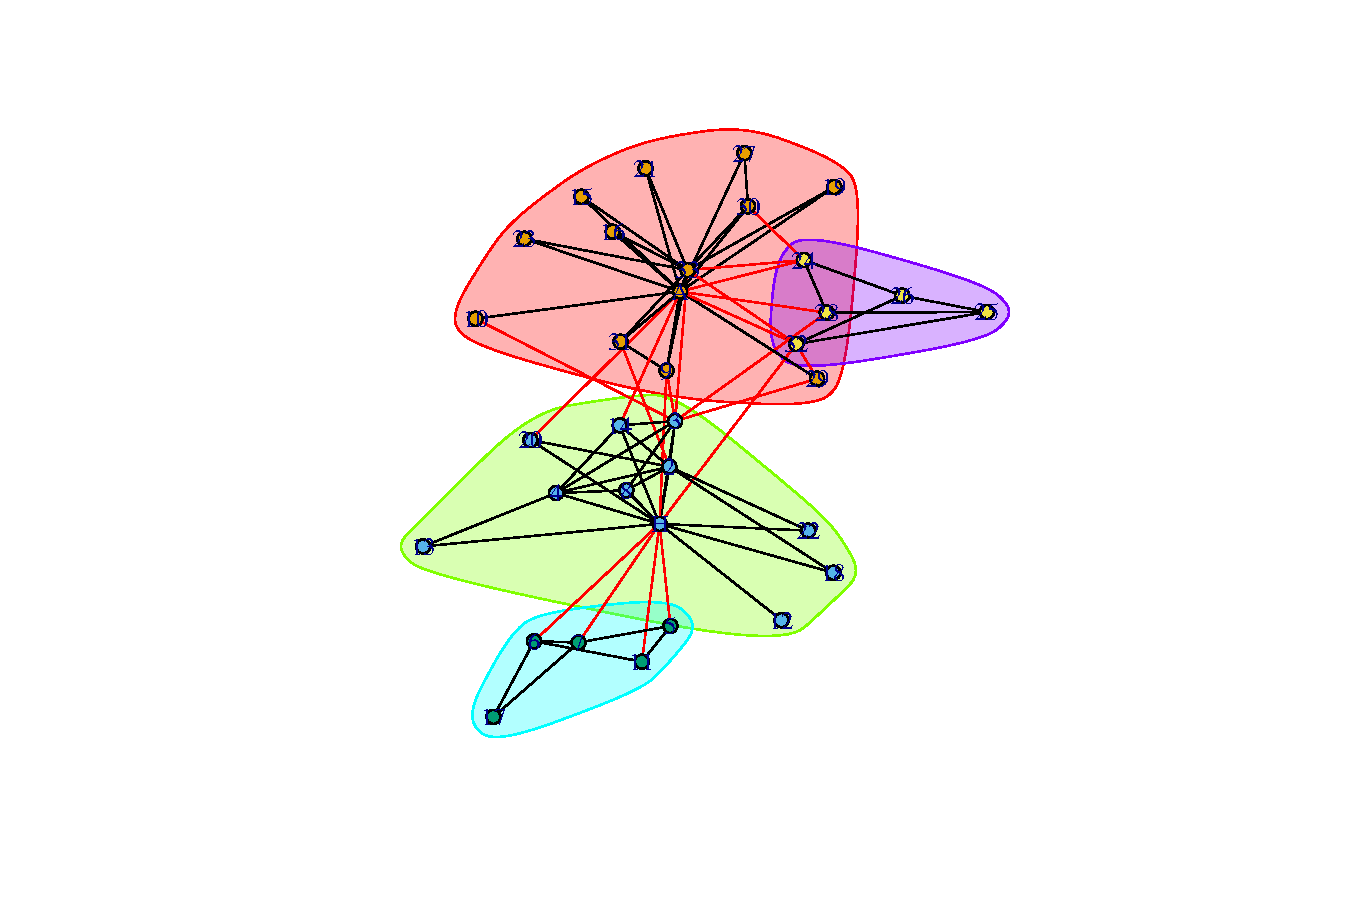
\includegraphics[width=.8\textwidth]{figures/unnamed-chunk-6-1} 

\end{knitrout}

\end{frame}

%% ==========================================================================
%% ==========================================================================
\section{The Stochastic Block Model (SBM)}
%% ==========================================================================

\begin{frame}
  \frametitle{Motivations}

  \begin{block}{Previous Section: \alert{find an underlying organization in a observed network}}
    Spectral or hierachical clustering for network data \\
    \begin{itemize}
      \item[$\rightsquigarrow$] \alert{Not model-based}, thus no statistical inference possible
    \end{itemize}
  \end{block}

  \begin{block}{This Section: \alert{clustering of network based on a probabilistic model of the graph}}<2->
    Become familiar with
    \begin{itemize}
      \item the stochastic block model, a random graph model tailored for clustering vertices
    \end{itemize}
  \end{block}

  \onslide<3>{
  \begin{center}
    hierarchical clustering $\leftrightarrow$ \alert{Gaussian mixture models} \\
      $\Updownarrow$ \\
    hierarchical/spectral clustering for network $\leftrightarrow$ Stochastic block model
  \end{center}
  }
\end{frame}

%% ==========================================================================
\subsection{Some Graphs Models and their limitations}
%% ==========================================================================

\begin{frame}
  \frametitle{A mathematical model: Erdös-Rényi graph}

  \begin{definition}
    Let $\clV = {1,\dots,n}$ be a set of fixed vertices. The (simple) Erdös-Rény model $\mathcal{G}(n,\pi)$ assumes random edges between pairs of nodes with probability $\pi$. In orther word, the (random) adjacency matrix $\bX$ is such that
    \begin{equation*}
      X_{ij} \sim \mathcal{B}(\pi)
    \end{equation*}
  \end{definition}

  \vfill

  \begin{proposition}[degree distribution]
    The (random) degree $D_i$ of vertex $i$ follows a binomial distribution:
      \begin{equation*}
        D_i \sim b(n-1, \pi).
      \end{equation*}
  \end{proposition}

\end{frame}

\begin{frame}[fragile]
  \frametitle{Erdös-Rényi - example}

\begin{knitrout}\scriptsize
\definecolor{shadecolor}{rgb}{0.969, 0.969, 0.969}\color{fgcolor}\begin{kframe}
\begin{alltt}
\hlstd{G1} \hlkwb{<-} \hlstd{igraph}\hlopt{::}\hlkwd{sample_gnp}\hlstd{(}\hlnum{10}\hlstd{,} \hlnum{0.1}\hlstd{)}
\hlstd{G2} \hlkwb{<-} \hlstd{igraph}\hlopt{::}\hlkwd{sample_gnp}\hlstd{(}\hlnum{10}\hlstd{,} \hlnum{0.9}\hlstd{)}
\hlstd{G3} \hlkwb{<-} \hlstd{igraph}\hlopt{::}\hlkwd{sample_gnp}\hlstd{(}\hlnum{100}\hlstd{,} \hlnum{.02}\hlstd{)}
\hlkwd{par}\hlstd{(}\hlkwc{mfrow}\hlstd{=}\hlkwd{c}\hlstd{(}\hlnum{1}\hlstd{,}\hlnum{3}\hlstd{))}
\hlkwd{plot}\hlstd{(G1,} \hlkwc{vertex.label}\hlstd{=}\hlnum{NA}\hlstd{) ;} \hlkwd{plot}\hlstd{(G2,} \hlkwc{vertex.label}\hlstd{=}\hlnum{NA}\hlstd{)}
\hlkwd{plot}\hlstd{(G3,} \hlkwc{vertex.label}\hlstd{=}\hlnum{NA}\hlstd{,} \hlkwc{layout}\hlstd{=layout.circle)}
\end{alltt}
\end{kframe}
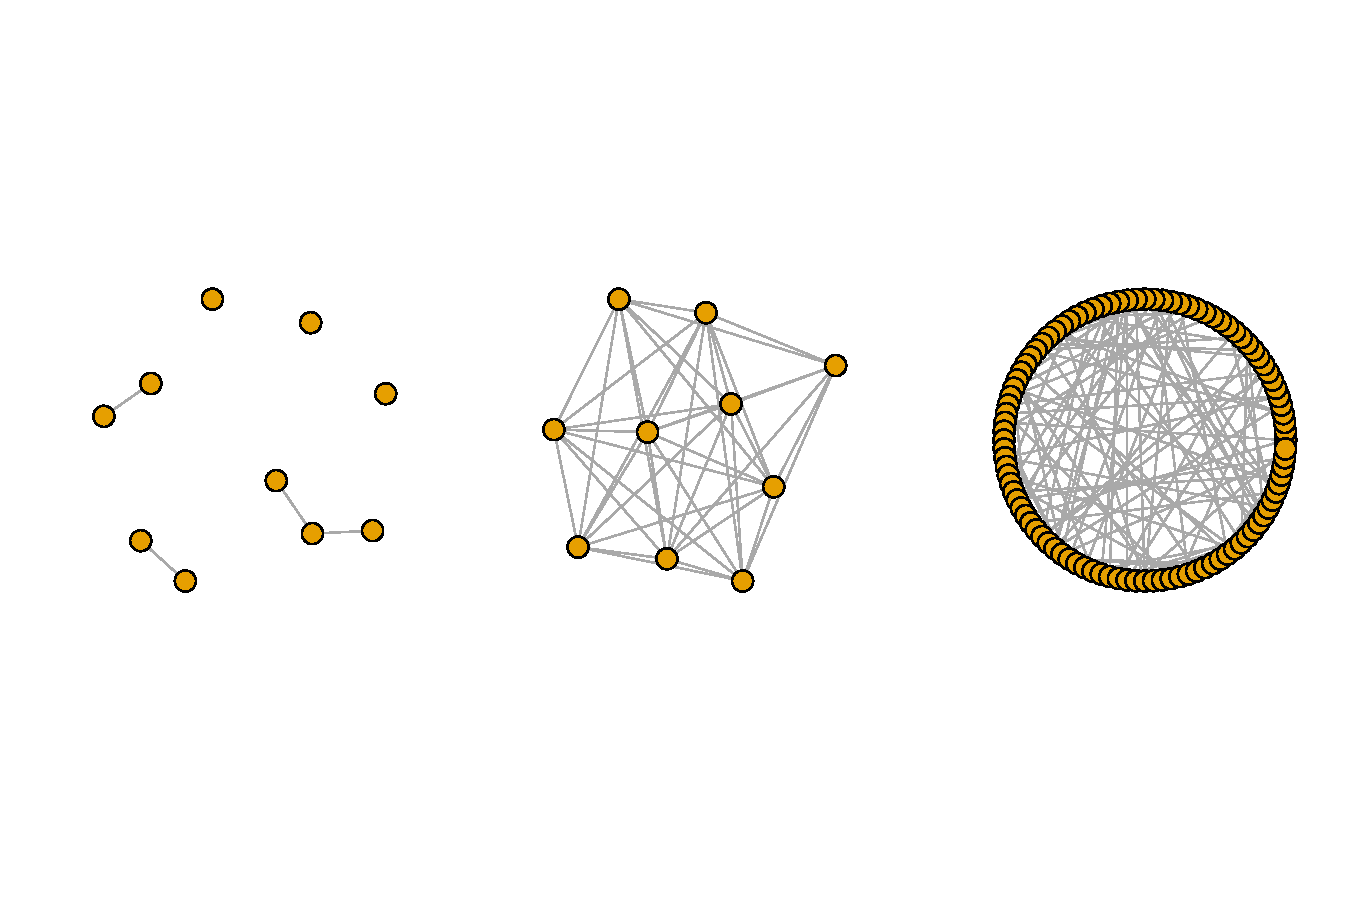
\includegraphics[width=.8\textwidth]{figures/ER_example-1} 

\end{knitrout}
\end{frame}

\begin{frame}[fragile]
  \frametitle{Erdös-Rény - limitations: very homegeneous}

\begin{knitrout}\scriptsize
\definecolor{shadecolor}{rgb}{0.969, 0.969, 0.969}\color{fgcolor}\begin{kframe}
\begin{alltt}
\hlkwd{average.path.length}\hlstd{(G3);} \hlkwd{diameter}\hlstd{(G3)}
\end{alltt}
\begin{verbatim}
## [1] 4.642086
## [1] 10
\end{verbatim}
\end{kframe}
\end{knitrout}

\begin{knitrout}\scriptsize
\definecolor{shadecolor}{rgb}{0.969, 0.969, 0.969}\color{fgcolor}
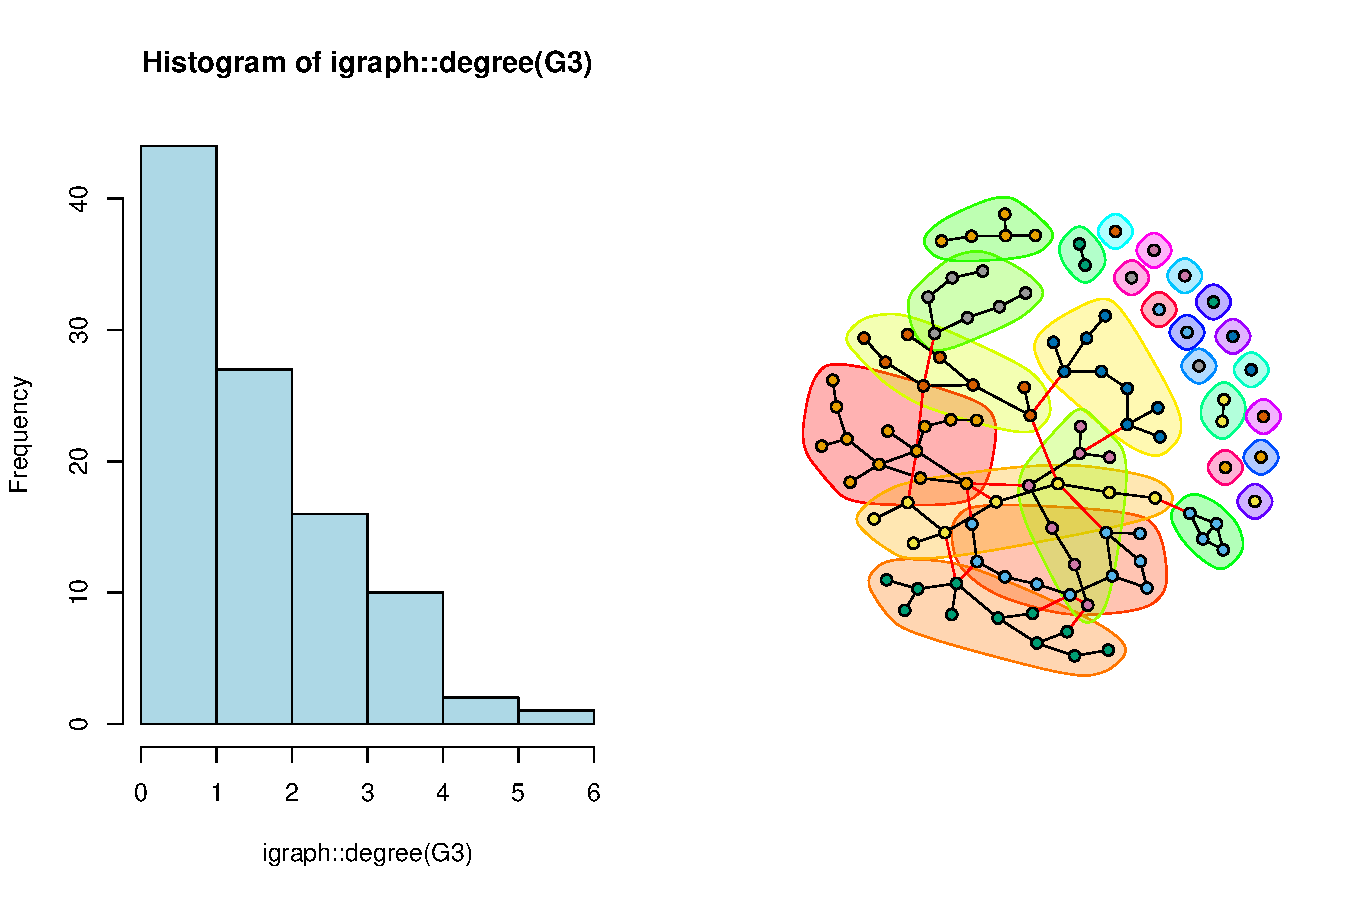
\includegraphics[width=.8\textwidth]{figures/ER_limitation2-1} 

\end{knitrout}
\end{frame}

% \begin{frame}
%   \frametitle{Mechanism-based model: preferential attachment}
% 
%   The graph is defined dynamically as follows
%   \begin{block}{Definition}
%     Start from a initial graph $\mathcal{G}_0 = (\mathcal{V}_0,\mathcal{E}_0)$, then for each time step,
%     \begin{enumerate}
%       \item At $t$ a new node $V_t$ is added
%       \item $V_t$ is connected to $i \in V_{t-1}$ with probability
%       \begin{equation*}
%         D_i^\alpha + \mathrm{cst.}
%       \end{equation*}
%     \end{enumerate}
%   \end{block}
%   $\rightsquigarrow$ Nodes with high degree get more connections thus \alert{richers get richers}
% \end{frame}
% 
% \begin{frame}[fragile]
%   \frametitle{Preferential attachment - example}
% 
% <<PA_example>>=
% G1 <- igraph::sample_pa(20, 1, directed=FALSE)
% G2 <- igraph::sample_pa(20, 5, directed=FALSE)
% G3 <- igraph::sample_pa(200, directed=FALSE)
% par(mfrow=c(1,3))
% plot(G1, vertex.label=NA) ; plot(G2, vertex.label=NA)
% plot(G3, vertex.label=NA, layout=layout.circle)
% @
% 
% \end{frame}
% 
% \begin{frame}[fragile]
%   \frametitle{Preferential attachment - limitations}
% 
% <<PA_limitation1>>=
% average.path.length(G3); diameter(G3)
% @
% 
% <<PA_limitation2, echo=FALSE>>=
% par(mfrow=c(1,2))
% hist(degree(G3), col="lightblue"); plot(cluster_fast_greedy(G3), G3)
% @
% \end{frame}

\begin{frame}
  \frametitle{Limitations}

    \begin{itemize}
    \item \alert{Erdös-Rényi}\\
      The ER model does not fit well real world network
      \begin{itemize}
        \item As can been seen from its degree distribution
        \item ER is generally too homogeneous
      \end{itemize}
    \end{itemize}

  \vfill

  \begin{block}{The Stochastic Block Model}
    The SBM\footnote{Other models exist (e.g. exponential model for random graphs) but less popular.} generalizes ER in a mixture framework. It provides
    \begin{itemize}
      \item a statistical framework to adjust and interpret the parameters
      \item a flexible yet simple specification that fits many existing network data
    \end{itemize}
  \end{block}

\end{frame}


%% ==========================================================================
\subsection{Mixture of Erdös-Rényi and the SBM}
%% ==========================================================================

\begin{frame}
  \frametitle{Stochastic Block Model: definition}
    \framesubtitle{Mixture model point of view: mixture of Erdös-Rényi}

    \begin{block}{Latent structure}
      Let $\mathcal{V} = \set{1,..,n}$ be a fixed set of vertices. We give each $i\in\mathcal{V}$ a \alert{latent label} among a set $\mathcal{Q}=\{1,\dots,Q\}$ such that
    \begin{itemize}
    \item $\alpha_q = \prob(i\in q), \quad \sum_q \alpha_q=1$;
    \item $Z_{iq}=\1_{\{i \in  q\}}$  are independent  hidden variables.
   \end{itemize}
   \end{block}

    \begin{block}{The conditional distribution of the edges}
    Connexion probabilities depend on the node class belonging:
    \begin{equation*}
      X_{ij} | \set{i\in q, j\in\ell} \sim \mathcal{B}(\pi_{q \ell}) \qquad \bigg(\Leftrightarrow       X_{ij} | \set{Z_{iq}Z_{j\ell}=1} \sim \mathcal{B}(\pi_{q \ell}).
 \bigg)
    \end{equation*}
    The $Q\times Q$ matrix ${\boldsymbol\pi}$  gives for all couple of labels $\pi_{q\ell}=\mathbb{P}(X_{ij}=1|i\in q, j\in\ell)$.
   \end{block}

\end{frame}


\begin{frame}
  \frametitle{Stochastic Block Model: the big picture}

  \begin{center}
    \begin{overlayarea}{\textwidth}{.5\textheight}
      \begin{columns}
        \begin{column}{.45\paperwidth}
        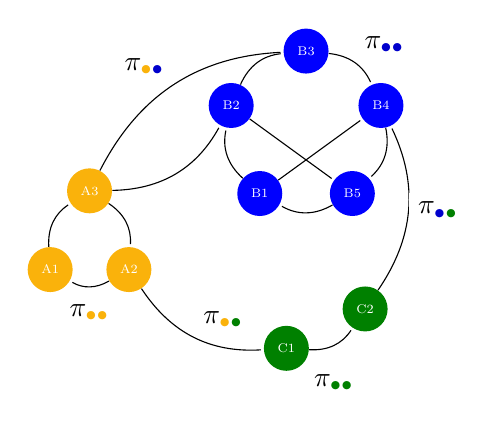
\begin{tikzpicture}
          %% UN GRAPH

          \tikzstyle{every edge}=[-,>=stealth',shorten >=1pt,auto,thin,draw]
          \tikzstyle{every state}=[draw=none,text=white,scale=0.65, font=\scriptsize, transform shape]
          \tikzstyle{every node}=[fill=yellow!40!orange]
          % premier cluster
          \node[state] (A1) at (0,0.5) {A1};
          \node[state] (A2) at (1,0.5) {A2};
          \node[state] (A3) at (.5,1.5) {A3};

          \path (A2) edge [bend left] node[fill=white,below=.1cm]
          {$\pi_{\textcolor{yellow!40!orange}{\bullet}\textcolor{yellow!40!orange}{\bullet}}$}
          (A1)
          (A1) edge [bend left] (A3)
          (A3) edge [bend left] (A2);

          \tikzstyle{every node}=[fill=blue!80!black]
          \foreach \angle/\text in {234/B1, 162/B2, 90/B3, 18/B4, -54/B5} {
            \node[fill=blue,state,xshift=5cm,yshift=3.5cm]     (\text)    at
            (\angle:1cm) {\text};
          }
          \path (B2) edge (B5)
          (B1) edge (B4);
          \foreach \from/\to in {1/2,2/3,4/5,5/1}{
            \path (B\from) edge [bend left] (B\to);
          }

          \path    (B3)    edge     [bend    left]    node[fill=white]
          {$\pi_{\textcolor{blue!80!black}{\bullet}\textcolor{blue!80!black}{\bullet}}$}  (B4) ;

          \tikzstyle{every node}=[fill=green!50!black]
          % troisieme cluster
          \node[state] (C1) at (3,-.5) {C1};
          \node[state] (C2) at (4,0) {C2};

          \path (C1) edge [bend right] node[fill=white,below=.25cm]
          {$\pi_{\textcolor{green!50!black}{\bullet}\textcolor{green!50!black}{\bullet}}$}
          (C2);

          % inter cluster
          \path (A3) edge [bend right]  (B2)
          (A3)    edge    [bend    left]    node[fill=white]
          {$\pi_{\textcolor{yellow!40!orange}{\bullet}\textcolor{blue!80!black}{\bullet}}$}
          (B3)
          (C2) edge [bend right] node[fill=white,right]
          {$\pi_{\textcolor{blue!80!black}{\bullet}\textcolor{green!50!black}{\bullet}}$}
          (B4)
          (A2) edge [bend right] node[fill=white]
          {$\pi_{\textcolor{yellow!40!orange}{\bullet}\textcolor{green!50!black}{\bullet}}$}
          (C1);
        \end{tikzpicture}
        \end{column}
        \begin{column}{.5\paperwidth}
          \begin{small}
            \begin{block}{Stochastic Block Model}
              Let $n$ nodes divided into
              \begin{itemize}
              \item
                $\mathcal{Q}=\{\textcolor{yellow!40!orange}{\bullet},\textcolor{blue!80!black}{\bullet},\textcolor{green!50!black}{\bullet}\}$
                classes
              \item  $\alpha_\bullet  =  \mathbb{P}(i  \in  \bullet)$,
                $\bullet\in\mathcal{Q},i=1,\dots,n$
              \item      $\pi_{\textcolor{yellow!40!orange}{\bullet}\textcolor{blue!80!black}{\bullet}}     =      \mathbb{P}(i
                \leftrightarrow j | i\in\textcolor{yellow!40!orange}{\bullet},j\in\textcolor{blue!80!black}{\bullet})$
              \end{itemize}
            \end{block}
          \end{small}
        \end{column}
      \end{columns}
    \end{overlayarea}
  \end{center}

  \begin{align*}
    Z_i = \mathbf{1}_{\{i \in \bullet\}}  \ & \sim^{\text{iid}} \mathcal{M}(1,\alpha), \quad \forall\bullet\in\mathcal{Q}, \\
    X_{ij} \ | \ \{i\in\textcolor{yellow!40!orange}{\bullet},j\in\textcolor{blue!80!black}{\bullet}\} & \sim^{\text{ind}} \mathcal{B}(\pi_{\textcolor{yellow!40!orange}{\bullet}\textcolor{blue!80!black}{\bullet}})\\
  \end{align*}

\end{frame}

\begin{frame}
  \frametitle{Stochastic Block Model: unknown parameters}

    \begin{center}
  \begin{overlayarea}{\textwidth}{.5\textheight}
      \begin{columns}
        \begin{column}{.45\paperwidth}
        \begin{tikzpicture}
          %% UN GRAPH

          \tikzstyle{every edge}=[-,>=stealth',shorten >=1pt,auto,thin,draw]
          \tikzstyle{every state}=[draw=none,text=white,scale=0.65, font=\scriptsize, transform shape]
          \tikzstyle{every node}=[fill=gray]
          % premier cluster
          \node[state] (A1) at (0,0.5) {N1};
          \node[state] (A2) at (1,0.5) {N2};
          \node[state] (A3) at (.5,1.5) {N3};

          \path (A2) edge [bend left] node[fill=white,below=.1cm]
          {}
          (A1)
          (A1) edge [bend left] (A3)
          (A3) edge [bend left] (A2);

          \tikzstyle{every node}=[fill=blue!80!black]
          \foreach \angle/\text in {234/N1, 162/N2, 90/N3, 18/N4, -54/N5} {
            \node[fill=gray,state,xshift=5cm,yshift=3.5cm]     (\text)    at
            (\angle:1cm) {\text};
          }
          \path (B2) edge (B5)
          (B1) edge (B4);
          \foreach \from/\to in {1/2,2/3,4/5,5/1}{
            \path (B\from) edge [bend left] (B\to);
          }

          \path (B3) edge [bend left] node[fill=white] {}  (B4) ;

          \tikzstyle{every node}=[fill=gray]
          % troisime cluster
          \node[state] (C1) at (3,-.5) {N1};
          \node[state] (C2) at (4,0) {N2};

          \path (C1) edge [bend right] (C2);

          % inter cluster
          \path (A3) edge [bend right]  (B2)
          (A3)    edge    [bend    left]    node[fill=white]
          {}
          (B3)
          (C2) edge [bend right] node[fill=white,right]
          {}
          (B4)
          (A2) edge [bend right] node[fill=white]
          {}
          (C1);
        \end{tikzpicture}
        \end{column}
        \begin{column}{.5\paperwidth}
          \begin{small}
            \begin{block}{Stochastic Block Model}
              Let $n$ nodes divided into
              \begin{itemize}
              \item
                $\mathcal{Q}=\{\textcolor{yellow!40!orange}{\bullet},\textcolor{blue!80!black}{\bullet},\textcolor{green!50!black}{\bullet}\}$,
                $\text{card}(\mathcal{Q})$ known
              \item  $\alpha_\bullet  =  ?$,
              \item      $\pi_{\textcolor{yellow!40!orange}{\bullet}\textcolor{blue!80!black}{\bullet}}     =      ?$
              \end{itemize}
            \end{block}
          \end{small}
        \end{column}
      \end{columns}
    \end{overlayarea}
    \end{center}

  \begin{align*}
    Z_i = \mathbf{1}_{\{i \in \bullet\}}  \ & \sim^{\text{iid}} \mathcal{M}(1,\alpha), \quad \forall\bullet\in\mathcal{Q}, \\
    X_{ij} \ | \ \{i\in\textcolor{yellow!40!orange}{\bullet},j\in\textcolor{blue!80!black}{\bullet}\} & \sim^{\text{ind}} \mathcal{B}(\pi_{\textcolor{yellow!40!orange}{\bullet}\textcolor{blue!80!black}{\bullet}})\\
  \end{align*}

\end{frame}

\begin{frame}[fragile]
  \frametitle{Stochastic block models -- examples of topology}
  \framesubtitle{Community network}

\begin{knitrout}\scriptsize
\definecolor{shadecolor}{rgb}{0.969, 0.969, 0.969}\color{fgcolor}\begin{kframe}
\begin{alltt}
\hlstd{pi} \hlkwb{<-} \hlkwd{matrix}\hlstd{(}\hlkwd{c}\hlstd{(}\hlnum{0.3}\hlstd{,}\hlnum{0.02}\hlstd{,}\hlnum{0.02}\hlstd{,}\hlnum{0.02}\hlstd{,}\hlnum{0.3}\hlstd{,}\hlnum{0.02}\hlstd{,}\hlnum{0.02}\hlstd{,}\hlnum{0.02}\hlstd{,}\hlnum{0.3}\hlstd{),}\hlnum{3}\hlstd{,}\hlnum{3}\hlstd{)}
\hlstd{communities} \hlkwb{<-} \hlstd{igraph}\hlopt{::}\hlkwd{sample_sbm}\hlstd{(}\hlnum{100}\hlstd{, pi,} \hlkwd{c}\hlstd{(}\hlnum{25}\hlstd{,} \hlnum{50}\hlstd{,} \hlnum{25}\hlstd{))}
\hlkwd{plot}\hlstd{(communities,} \hlkwc{vertex.label}\hlstd{=}\hlnum{NA}\hlstd{,} \hlkwc{vertex.color} \hlstd{=} \hlkwd{rep}\hlstd{(}\hlnum{1}\hlopt{:}\hlnum{3}\hlstd{,}\hlkwd{c}\hlstd{(}\hlnum{25}\hlstd{,} \hlnum{50}\hlstd{,} \hlnum{25}\hlstd{)))}
\end{alltt}
\end{kframe}
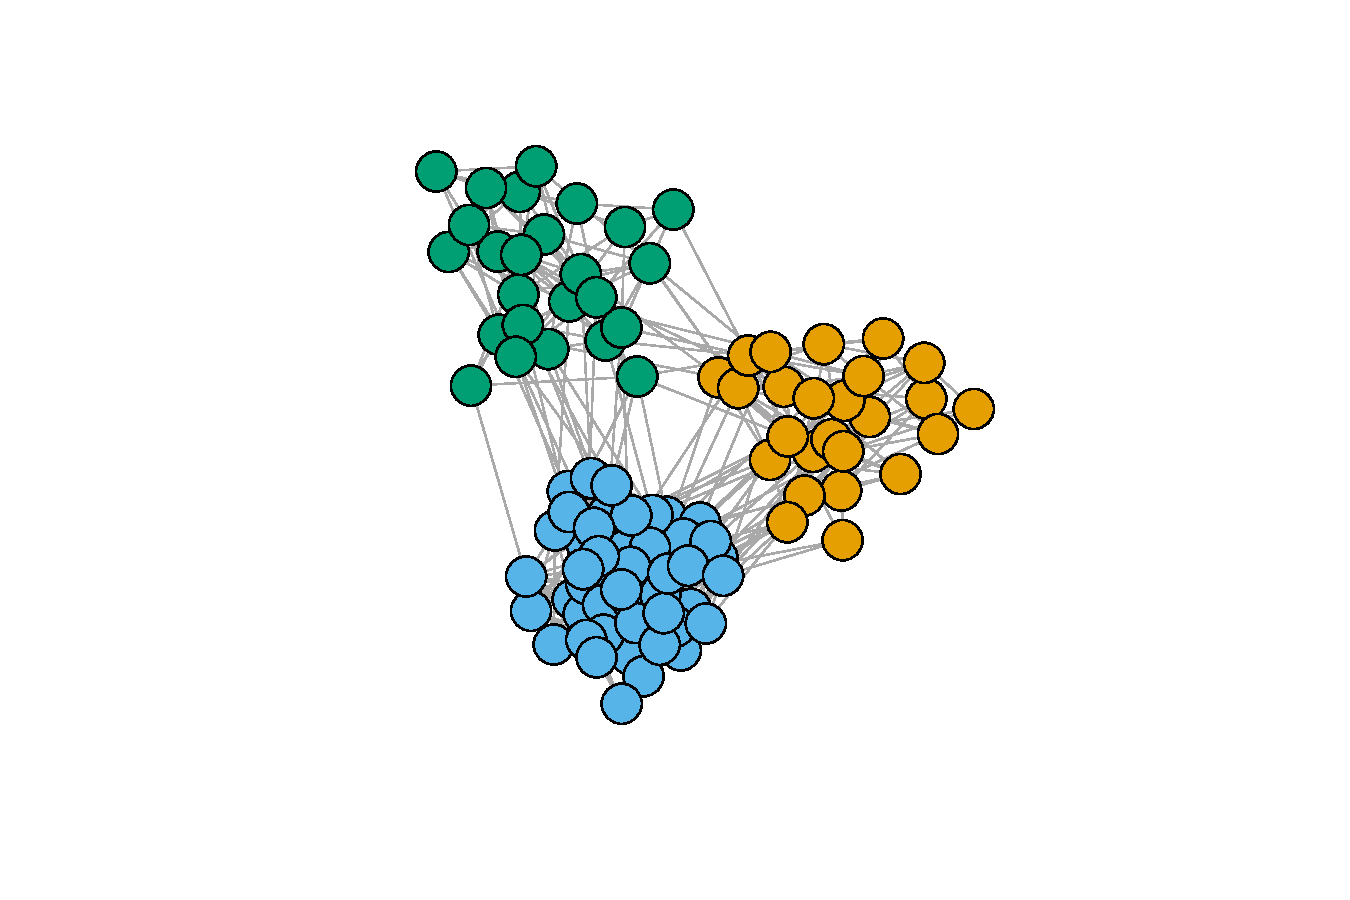
\includegraphics[width=.8\textwidth]{figures/unnamed-chunk-7-1} 

\end{knitrout}

\end{frame}

\begin{frame}[fragile]
  \frametitle{Stochastic block models -- examples of topology}
  \framesubtitle{Star network}

\begin{knitrout}\scriptsize
\definecolor{shadecolor}{rgb}{0.969, 0.969, 0.969}\color{fgcolor}\begin{kframe}
\begin{alltt}
\hlstd{pi} \hlkwb{<-} \hlkwd{matrix}\hlstd{(}\hlkwd{c}\hlstd{(}\hlnum{0.05}\hlstd{,}\hlnum{0.3}\hlstd{,}\hlnum{0.3}\hlstd{,}\hlnum{0}\hlstd{),}\hlnum{2}\hlstd{,}\hlnum{2}\hlstd{)}
\hlstd{star} \hlkwb{<-} \hlstd{igraph}\hlopt{::}\hlkwd{sample_sbm}\hlstd{(}\hlnum{100}\hlstd{, pi,} \hlkwd{c}\hlstd{(}\hlnum{4}\hlstd{,} \hlnum{96}\hlstd{))}
\hlkwd{plot}\hlstd{(star,} \hlkwc{vertex.label}\hlstd{=}\hlnum{NA}\hlstd{,} \hlkwc{vertex.color} \hlstd{=} \hlkwd{rep}\hlstd{(}\hlnum{1}\hlopt{:}\hlnum{2}\hlstd{,}\hlkwd{c}\hlstd{(}\hlnum{4}\hlstd{,}\hlnum{96}\hlstd{)))}
\end{alltt}
\end{kframe}
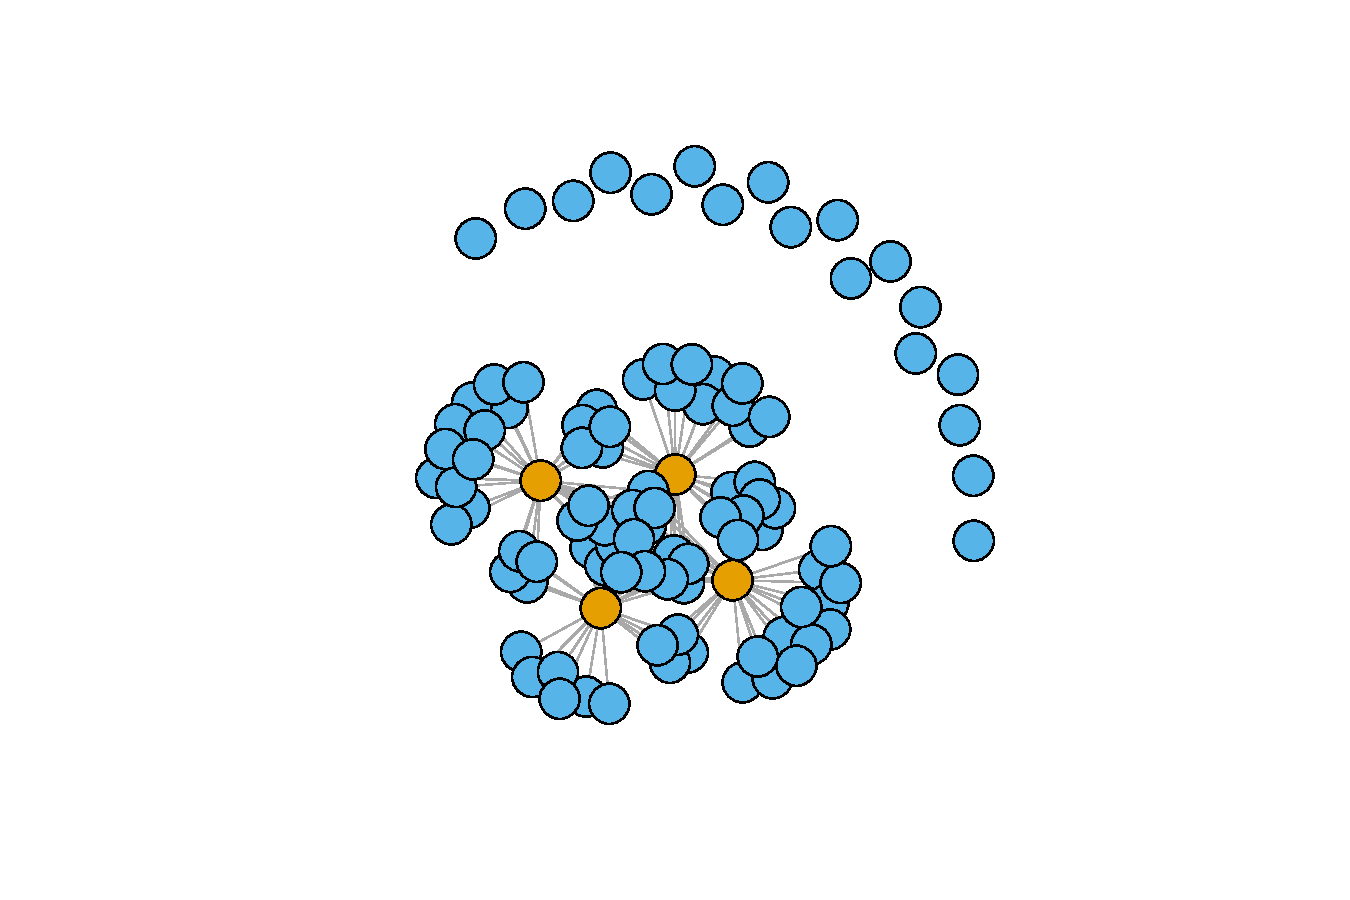
\includegraphics[width=.8\textwidth]{figures/unnamed-chunk-8-1} 

\end{knitrout}

\end{frame}

% \begin{frame}
%   \frametitle{Degree distributions}
% 
%   \begin{block}{Conditional degree distribution}
%     The conditional degree distribution of a node $i\in q$ is
%     \begin{equation*}
%       D_i | i \in q \sim \mathrm{b}(n-1,\bar\pi) \approx \mathcal{P}(\lambda_q), \qquad \bar\pi_q = \sum_{\ell=1}^Q \alpha_\ell, \pi_{q\ell} \quad \lambda_q = (n-1)\bar\pi_q
%     \end{equation*}
%   \end{block}
% 
%   \vfill
% 
%   \begin{block}{Conditional degree distribution}
%     The degree distribution of a node $i$ can be approximated by a mixture of Poisson distributions:
%     \begin{equation*}
%       \prob(D_i = k) = \sum_{q=1}^Q\alpha_q \exp{\set{-\lambda_q}} \ \frac{\lambda_q^k}{k !}
%     \end{equation*}
%   \end{block}
% 
% \end{frame}
% 

\begin{frame}
  \frametitle{Likelihoods for Expectation Maximization}

  \begin{block}{Complete-data loglikelihood}
    \vspace{-.5cm}
    \begin{equation*}
      \log L(\bX,\bZ) = \sum_{i,q} Z_{iq} \log \alpha_q + \sum_{i<j,q,\ell} Z_{iq}Z_{j\ell} \log \pi_{q\ell}^{X_{ij}} (1-\pi_{q\ell})^{1-X_{ij}}.
    \end{equation*}
  \end{block}

  \begin{block}{Conditional expectation of the complete-data loglikelihood}
    \vspace{-.5cm}
    \begin{equation*}
      \E_{\bZ|\bX} \big[\log L(\btheta;\bX,\bZ) \big] = \sum_{i,q} \tau_{iq} \log \alpha_q + \sum_{i<j,q,\ell} \eta_{ijq\ell} \log \pi_{q\ell}^{X_{ij}} (1-\pi_{q\ell})^{1-X_{ij}}
    \end{equation*}
      where $\tau_ {iq}, \eta_{ijq\ell}$ are the posterior probabilities:
      \begin{itemize}
        \item $\tau_{iq} = \prob(Z_{iq} = 1 | \bX) = \E \left[Z_{iq} | \bX\right].$
        \item $\eta_{ijq\ell} = \prob(Z_{iq}Z_{j\ell} = 1 | \bX) = \E \left[Z_{iq}Z_{j\ell} | \bX\right].$
      \end{itemize}
  \end{block}

\end{frame}

\begin{frame}
  \frametitle{Inference in the SBM}
  \framesubtitle{The EM strategy does not apply}
  
  \begin{block}{Ouch: another intractability problem}
    \begin{itemize}
      \item the $Z_{iq}$ are \alert{not independent} in the SBM framework\dots
      \item we cannot compute $\eta_{ijq\ell} = \prob(Z_{iq}Z_{j\ell} = 1 | \bX) = \E \left[Z_{iq}Z_{j\ell} | \bX\right]$,
      \item the conditional expectation $Q(\btheta)$, i.e. the main EM ingredient, is \alert{intractable}.
    \end{itemize}
  \end{block}

  \vfill

  \begin{block}{Solution: mean field approximation (variational inference)}
    Approximate $\eta_{ijq\ell}$ by $\tau_{iq}\tau_{j\ell}$, i.e., \alert{assume independence between $Z_{iq}$}\\

    $\rightsquigarrow$ This can be formalized in the variational framework
  \end{block}


\end{frame}

\begin{frame}
  \frametitle{Model selection: the number of blocks/clusters}

  We use our lower bound of the  loglikelihood to compute an approximation of the ICL
  \begin{multline*}
  \mathrm{vICL}(Q) = \E_{\hat{\mathbb{Q}}} [\log L(\hat{\btheta)};\bX,\bZ] \\ - \frac{1}{2} \left(\frac{Q(Q+1)}{2} \log \frac{n(n-1)}{2} + (Q-1) \log (n) \right),
\end{multline*}
where
    \begin{equation*}
      \E_{\hat{\mathbb{Q}}} [\log L(\hat\btheta; \bX,\bZ)] = J(\hat{\boldsymbol\tau},\hat\btheta) - \mathcal{H}(\hat{\mathbb{Q}}).
    \end{equation*}

    The variational BIC is just
    \begin{equation*}
  \mathrm{vBIC}(Q) = J(\hat{\boldsymbol\tau},\hat\btheta) - \frac{1}{2} \left(\frac{Q(Q+1)}{2} \log \frac{n(n-1)}{2} + (Q-1) \log (n) \right).
    \end{equation*}

\end{frame}

\begin{frame}[fragile]
  \frametitle{Example on the French blogsphere (I)}

\begin{knitrout}\scriptsize
\definecolor{shadecolor}{rgb}{0.969, 0.969, 0.969}\color{fgcolor}\begin{kframe}
\begin{alltt}
\hlkwd{library}\hlstd{(blockmodels)}
\hlkwd{library}\hlstd{(sand)}

\hlstd{adj_blog} \hlkwb{<-} \hlkwd{upgrade_graph}\hlstd{(fblog)} \hlopt
    \hlkwd{as_adjacency_matrix}\hlstd{()} \hlopt
    \hlkwd{as.matrix}\hlstd{()}

\hlstd{mySBM_collection} \hlkwb{<-} \hlkwd{BM_bernoulli}\hlstd{(}
  \hlstr{"SBM_sym"}\hlstd{,}
  \hlstd{adj_blog,} \hlkwc{verbosity} \hlstd{=} \hlnum{0}\hlstd{,}
  \hlkwc{plotting} \hlstd{=} \hlstr{"figures/ICL_fblog.pdf"}
\hlstd{)}
\hlstd{mySBM_collection}\hlopt{$}\hlkwd{estimate}\hlstd{()}
\end{alltt}
\end{kframe}






































































\end{knitrout}

\end{frame}

\begin{frame}[fragile]
  \frametitle{Example on the French blogsphere (II)}

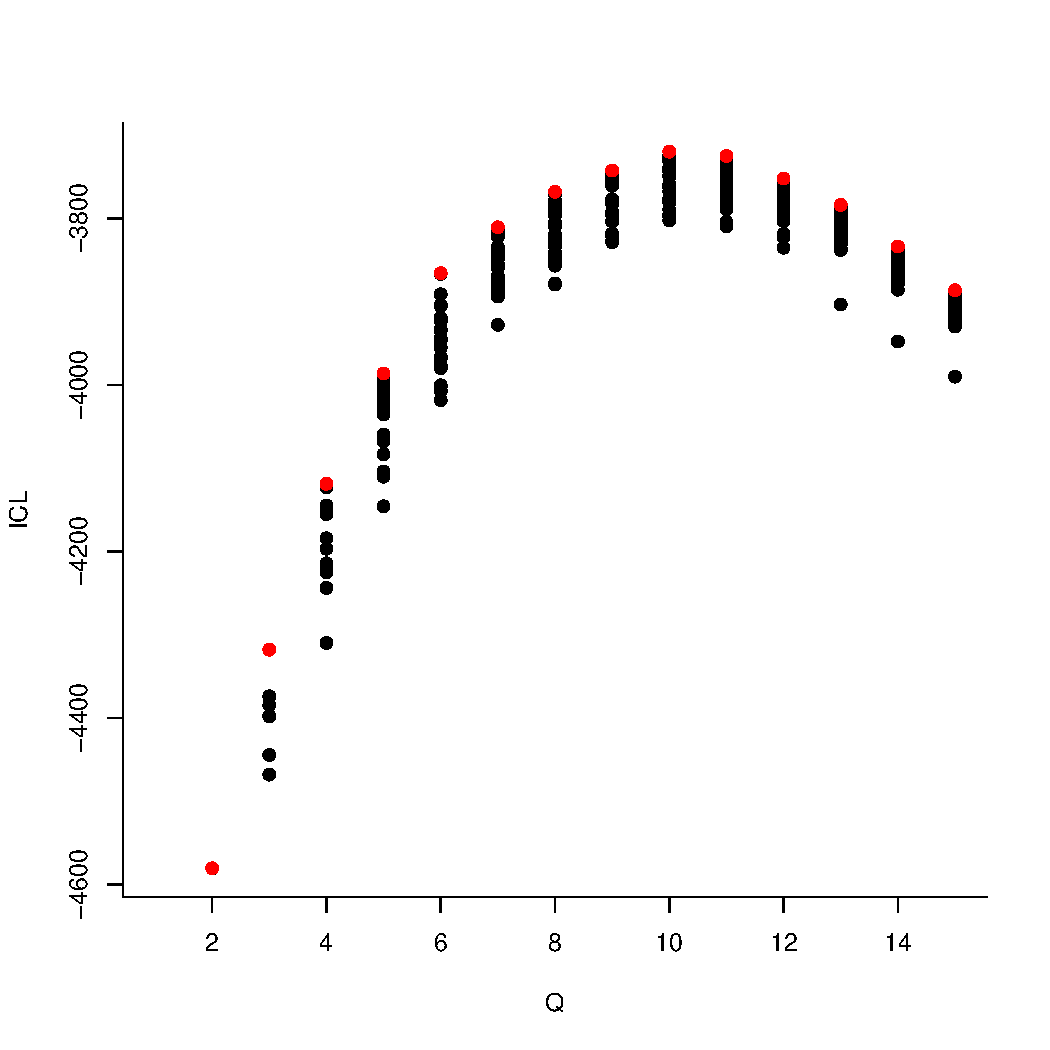
\includegraphics[width=.7\textwidth]{figures/ICL_fblog}

\end{frame}

\begin{frame}[fragile]
  \frametitle{Example on the French blogsphere (III)}

\begin{knitrout}\scriptsize
\definecolor{shadecolor}{rgb}{0.969, 0.969, 0.969}\color{fgcolor}\begin{kframe}
\begin{alltt}
\hlstd{clusters} \hlkwb{<-}
  \hlkwd{apply}\hlstd{(mySBM_collection}\hlopt{$}\hlstd{memberships[[}\hlnum{10}\hlstd{]]}\hlopt{$}\hlstd{Z,} \hlnum{1}\hlstd{, which.max)}
\hlkwd{image}\hlstd{(}\hlkwd{Matrix}\hlstd{(adj_blog[}\hlkwd{order}\hlstd{(clusters),} \hlkwd{order}\hlstd{(clusters)]))}
\end{alltt}
\end{kframe}
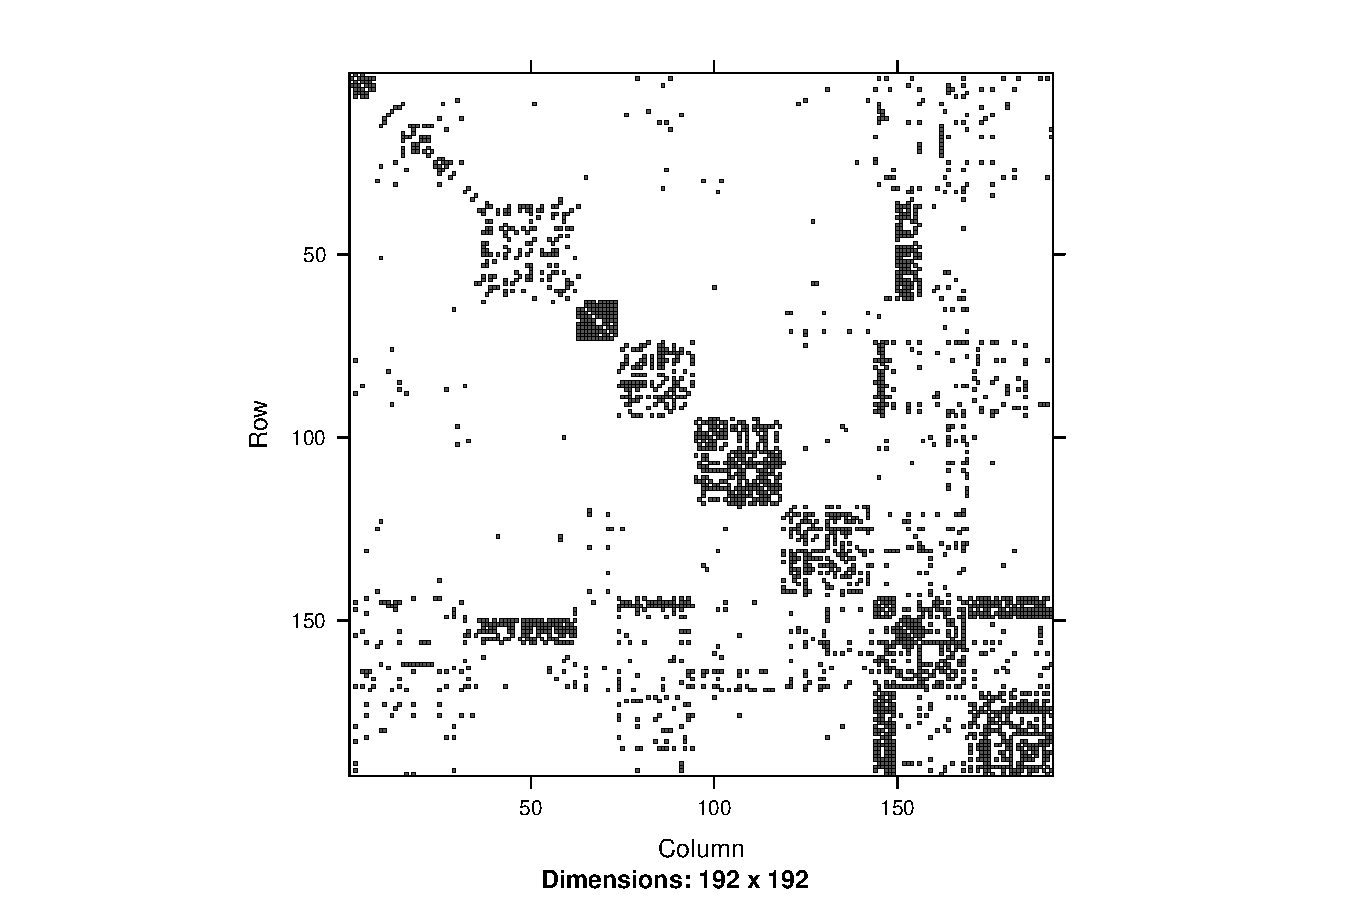
\includegraphics[width=.8\textwidth]{figures/example_blockmodels_3-1} 

\end{knitrout}

\end{frame}


\begin{frame}[fragile,allowframebreaks]
  \frametitle{Example on the French blogsphere (IV)}

\begin{knitrout}\scriptsize
\definecolor{shadecolor}{rgb}{0.969, 0.969, 0.969}\color{fgcolor}\begin{kframe}
\begin{alltt}
\hlkwd{library}\hlstd{(RColorBrewer); pal} \hlkwb{<-} \hlkwd{brewer.pal}\hlstd{(}\hlnum{10}\hlstd{,} \hlstr{"Set3"}\hlstd{)}

\hlstd{g} \hlkwb{<-} \hlkwd{graph_from_adjacency_matrix}\hlstd{(adj_blog,} \hlkwc{mode} \hlstd{=} \hlstr{"undirected"}\hlstd{,} \hlkwc{weighted} \hlstd{=} \hlnum{TRUE}\hlstd{,} \hlkwc{diag} \hlstd{=} \hlnum{FALSE}\hlstd{)}
\hlkwd{V}\hlstd{(g)}\hlopt{$}\hlstd{class} \hlkwb{<-} \hlstd{clusters}
\hlkwd{V}\hlstd{(g)}\hlopt{$}\hlstd{size} \hlkwb{<-} \hlnum{5}
\hlkwd{V}\hlstd{(g)}\hlopt{$}\hlstd{frame.color} \hlkwb{<-} \hlstr{"white"}
\hlkwd{V}\hlstd{(g)}\hlopt{$}\hlstd{color} \hlkwb{<-} \hlstd{pal[}\hlkwd{V}\hlstd{(g)}\hlopt{$}\hlstd{class]}
\hlkwd{V}\hlstd{(g)}\hlopt{$}\hlstd{label} \hlkwb{<-} \hlstr{""}
\hlkwd{E}\hlstd{(g)}\hlopt{$}\hlstd{arrow.mode} \hlkwb{<-} \hlnum{0}

\hlkwd{par}\hlstd{(}\hlkwc{mar} \hlstd{=}\hlkwd{c}\hlstd{(}\hlnum{0}\hlstd{,}\hlnum{0}\hlstd{,}\hlnum{0}\hlstd{,}\hlnum{0}\hlstd{))}
\hlkwd{plot}\hlstd{(g,} \hlkwc{edge.width}\hlstd{=}\hlkwd{E}\hlstd{(g)}\hlopt{$}\hlstd{weight)}
\end{alltt}
\end{kframe}

{\centering 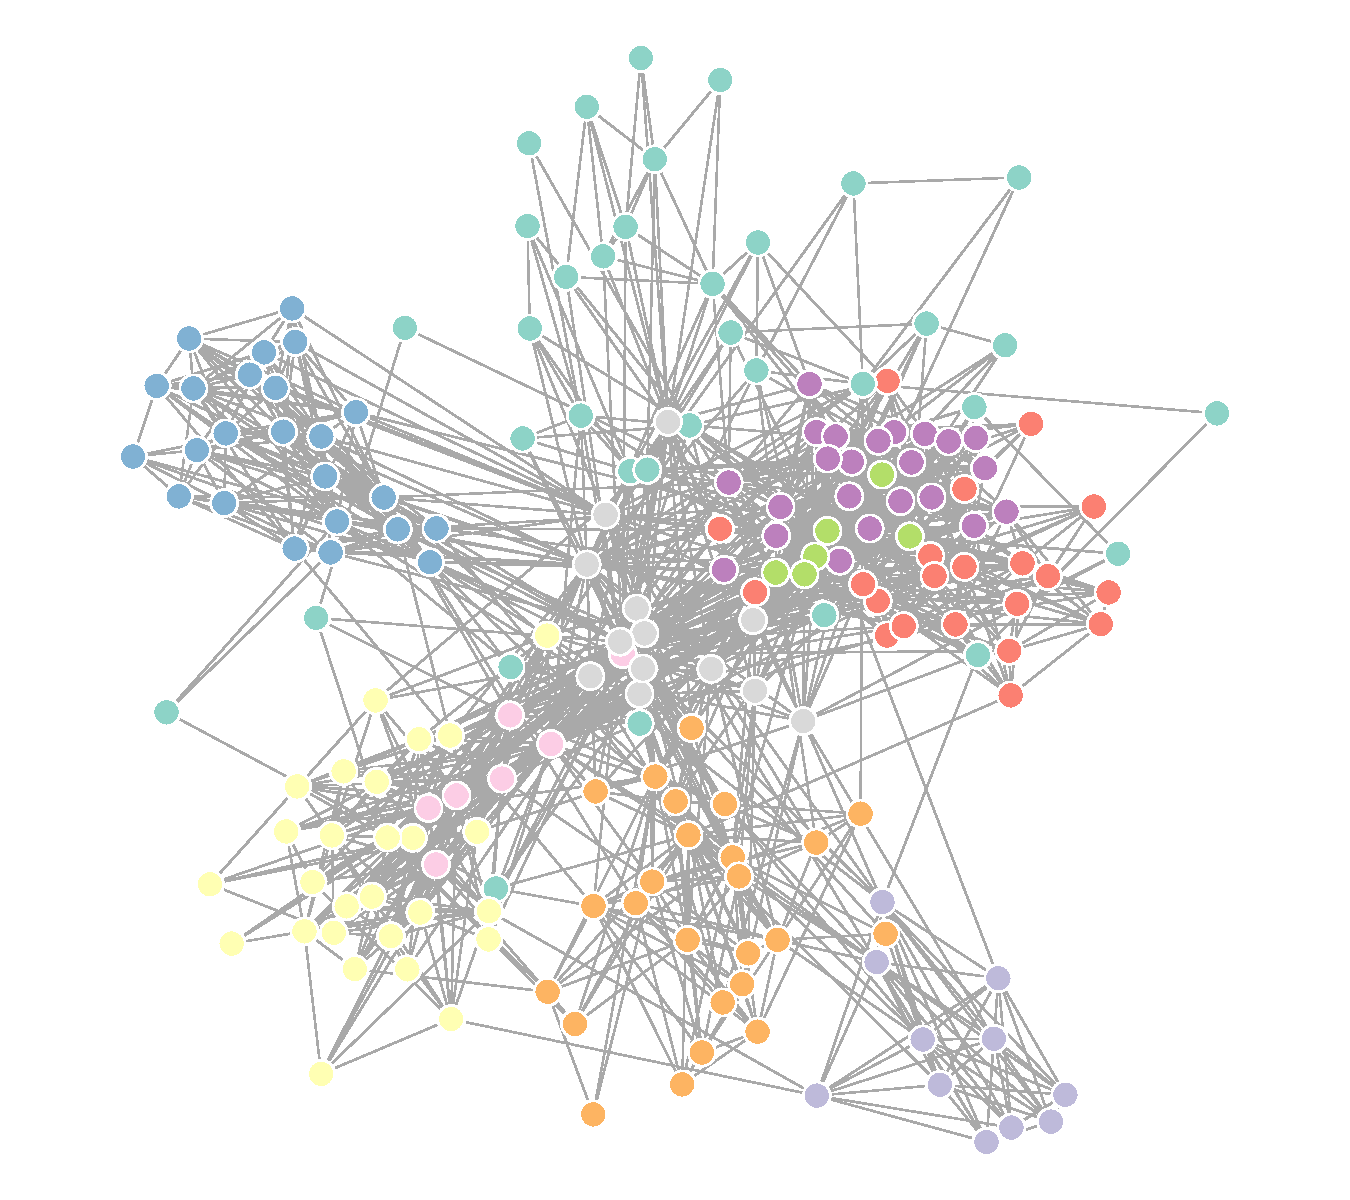
\includegraphics[width=.8\textwidth]{figures/example_blockmodels_4-1} 

}



\end{knitrout}

\end{frame}

\end{document}

